\chapter{Barren plateaus in variational algorithms}
\label{chap:plateaus}

In this chapter, we discuss the phenomenon of barren plateaus in VQAs. As the name suggests, the idea is that the optimization landscape of VQAs at randomly chosen points can often resemble a flat space with no good directions of search. This behavior of quantum circuits is in stark contrast with classical deep neural networks, where overparametrized neural networks are surprisingly good at finding good minima. We begin with technical details about random unitary operators and averaging over such operators. Then we move on to show how barren plateaus appear in generic overparametrized circuits. Finally, we report on our results regarding the barren plateaus in quantum circuits constructed out of small parametrized blocks, which are common in VQAs.

\section{Integration with respect to the Haar measure}

A typical ansatz quantum circuit is a large and complicated structure which is difficult to analyze. One way to study its properties is to analyze its average behavior with respect to sampling a random point in the parameter space. Such a sampling defines a probability measure on the unitary group $U(d)$\footnote{To specify the probability measure, you need the space of elementary outcomes $\Omega$ -- in our case, the group $U(d)$ -- and a certain algebra of its subsets called the Borel $\sigma$-algebra $\mathrm{Borel} (\Omega)$. A probability measure $P$ then has to map the subsets from $\mathrm{Borel} (\Omega)$ to $[0, 1]$ in a way that is (i) countably additive (ii) zero on the empty set and (iii) normalized: $P(\Omega) = 1$.}. 
It turns out that for many purposes this probability measure can be approximated by the probability measure on $U(d)$ called the Haar measure.

\begin{definition}
    The \textit{Haar measure} $\mu: \mathrm{Borel} (U(d)) \rightarrow [0, 1]$ on the unitary group $U(d)$ is the unique left- and right-invariant probability measure on that group. That is, let $V \in U(d)$ and let $\mathcal{A} \in \mathrm{Borel} (U(d))$. Then $\mu(\mathcal{A}) = \mu(V \mathcal{A}) = \mu(\mathcal{A} V)$.
\end{definition}

The proof that such measure is unique can be found e.g.~in \cite{watrous_theory_2018}.

In what follows, we will need to evaluate certain integrals over the unitary group. The integrands are related to matrix multiplications involving unitary matrices. As such, they will have the form of polynomials over the entries of $U$ and $U^*$. 

The simplest integral of that form is $\int U^\dagger A U \mathrm{d} \mu$. In tensor network diagrams, it can be expressed as follows:

\begin{equation}
    \label{eq:uau_picture}
    \int U^\dagger  A U  
    \mathrm{d} \mu
    = \int 
    % \includegraphics[valign=m,width=0.1\linewidth]
    % {
    \adjustbox{raise=2.5pt}{
    \Qcircuit @C=1em @R=.7em 
    {& \gate{U^\dagger} &  \gate{A} 
    & \gate{U} & \qw
    }
    }
    \ \mathrm{d} \mu.
\end{equation}

Here a wire means the vector space $\mathbb{C}^d$, not just a single-qubit space. We will also need a second-order integral of that sort:

\begin{equation}
    \label{eq:uuabuu_picture}
    \int (U^\dagger \otimes U^\dagger) (A \otimes B) (U \otimes U) 
    \mathrm{d} \mu
    = \int 
    % \includegraphics[valign=m,width=0.1\linewidth]
    % {
    \adjustbox{raise=15pt}{
    \Qcircuit @C=1em @R=.7em 
    {& \gate{U^\dagger} &  \gate{A} 
    & \gate{U} & \qw
    \\
    & \gate{U^\dagger} &  \gate{B} 
    & \gate{U} & \qw
    }
    }
    \mathrm{d} \mu.
\end{equation}

For more generality, we can consider integrals that don't use any additional matrices in their construction and just instead consider the following integral:

\begin{equation}
    \label{eq:unitary_integral}
    \mathcal{I}_t = \int U^{\otimes t} \otimes (U^\dagger)^{\otimes t} \mathrm{d} \mu.
\end{equation}

Note that when the tensor power of $U$ is not equal to the tensor power of $U^\dagger$, this integral is zero. This can be seen from the translation invariance of $\mu$. Let $V = e^{\mathrm{i}\theta} I$, then
\begin{equation}
    \int U^{\otimes t} \otimes (U^\dagger)^{\otimes t'} \mathrm{d} \mu
    = \int (VU)^{\otimes t} \otimes (U^\dagger V^\dagger)^{\otimes t'} \mathrm{d} \mu
    = e^{\mathrm{i}\theta (t - t')} \int U^{\otimes t} \otimes (U^\dagger)^{\otimes t'} \mathrm{d} \mu,
\end{equation}
which is possible only if $t = t'$ or if both sides of the equation are zero.


A tensor network diagram for this value is this:

\begin{equation}
    \label{eq:utut_picture}
    \mc{I}_t
    = \int 
    \adjustbox{valign=m}{
    \Qcircuit @C=1em @R=.7em 
    {& \gate{U} & \qw \\
    & \dots \\
    & \gate{U} & \qw \\
    & \gate{U^\dagger} & \qw \\
    & \dots \\
    & \gate{U^\dagger} & \qw \\
    }
    }
    \ \mathrm{d} \mu.
\end{equation}

The translation invariance of the Haar measure is the feature that enables us to calculate these integrals \cite{samuel_u_1980,collins_integration_2006}. Indeed, from the (left and right) translation invariance it follows that for any $V \in U(d)$, we have that 
\begin{align}
    \label{eq:haar_translation}
    (V^{\otimes t} \otimes \id^{\otimes t}) \mathcal{I}_t
    (\id^{\otimes t} \otimes (V^\dagger)^{\otimes t})  & = \mathcal{I}_t, \\
    (\id^{\otimes t} \otimes V^{\otimes t}) \mathcal{I}_t
    ((V^\dagger)^{\otimes t} \otimes \id^{\otimes t})  & = \mathcal{I}_t. 
\end{align}

In particular, the translation invariance implies \cite{samuel_u_1980} that $\mc{I}_t$ can only be a linear combination of permutations of tensor factors:

\begin{equation}
    \label{eq:haar_is_permutations}
    \mc{I}_t
    = \sum_{\sigma_A, \sigma_B \in S_t} C_{\sigma_A, \sigma_B}
    = \sum_{\sigma_A, \sigma_B \in S_t} C_{\sigma_A, \sigma_B}
    \adjustbox{raise=-40pt}{
    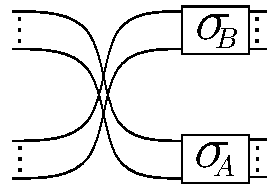
\includegraphics[width=0.25\linewidth]{figures/swap_and_perms.pdf}}
\end{equation}

The coefficients themselves are more difficult to obtain. We will restrict our attention to $t = 1$ and $t = 2$. The permutation group $S_1$ is trivial, so $\mathcal{I}_1 = c \cdot \mc{S}$. This implies that $\int U^\dagger A U \mathrm{d} \mu = (c \operatorname{Tr} A) \cdot I$:
\begin{equation}
    \label{eq:one_design_diagrams}
    \int 
    \adjustbox{raise=-3.5pt}{
    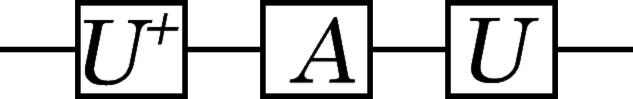
\includegraphics[width=0.15\linewidth]{figures/inkscape/uau_white_boxes.png}}
     \ \mathrm{d}\mu
    = \int 
    \adjustbox{raise=-8pt}{
    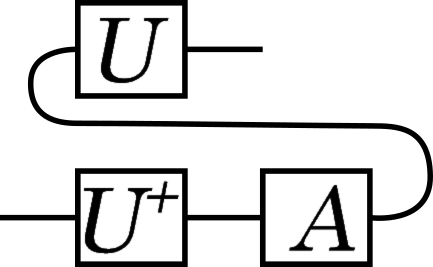
\includegraphics[width=0.1\linewidth]{figures/inkscape/uau_twist_white_boxes.png}} \ \mathrm{d}\mu
    = c \ \adjustbox{raise=-8pt}{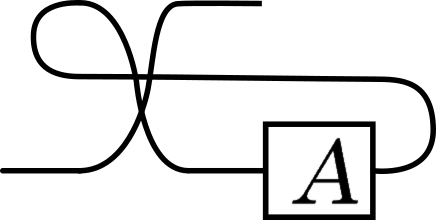
\includegraphics[width=0.12\linewidth]{figures/inkscape/swap_a_white_box.png}}
    = c \ \adjustbox{raise=-7pt}{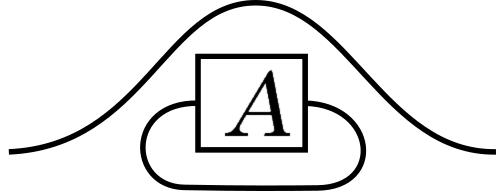
\includegraphics[width=0.12\linewidth]{figures/inkscape/tr_a_id_white_box.png}}
\end{equation}
The translation invariance implies that applying this unitary averaging twice will yield the same effect: $\int V^\dagger  U^\dagger A U V \mathrm{d}U \mathrm{d}V = \int U^\dagger A U \mathrm{d}U$. On the other hand, if we use (\ref{eq:one_design_diagrams}), we conclude that $c^2 \Tr \id \Tr A = c \Tr A$, which leads to $c = 1 / \Tr \id = 1/d$.


The case of $t = 2$ is somewhat more complicated. The group $S_2$ has two components, so the summation over $\{\sigma_A \times \sigma_B | \sigma_A, \sigma_B \in S_2\}$ has four terms:

\begin{equation}
    \mathcal{I}_2   
        = c_{II}\adjustbox{raise=-12pt}{
            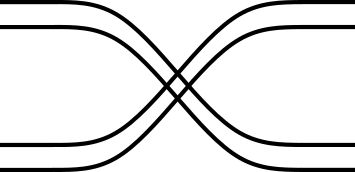
\includegraphics[width=0.12\linewidth]{figures/inkscape/ii.png}}
        + c_{IS}\adjustbox{raise=-12pt}{
            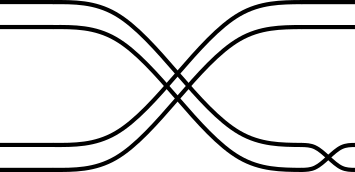
\includegraphics[width=0.12\linewidth]{figures/inkscape/is.png}}
        + c_{SI}\adjustbox{raise=-12pt}{
            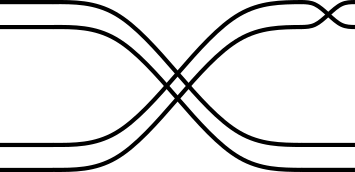
\includegraphics[width=0.12\linewidth]{figures/inkscape/si.png}}
        + c_{SS}\adjustbox{raise=-12pt}{
            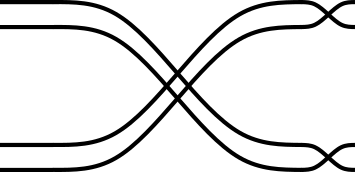
\includegraphics[width=0.12\linewidth]{figures/inkscape/ss.png}}.
\end{equation}

Now if we want to integrate $(U^\dagger \otimes U^\dagger) (A \otimes B) (U \otimes U)$ over $U$, we obtain the following formula:

\begin{multline}
    \label{eq:integrate_t2_no_coeffs}
    \int (U^\dagger \otimes U^\dagger) (A \otimes B) (U \otimes U) \mathrm{d} \mu = c_{II} (\Tr A \Tr B) \id \otimes \id +
    \\ + c_{SI} (\Tr A \Tr B) \mathcal{S} 
    + c_{IS} (\Tr AB) \id \otimes \id 
    + c_{SS} (\Tr AB) \mathcal{S}.
\end{multline}

The coefficients $c_{\sigma_A \sigma_B}$ here are no longer easy to calculate: the same trick as for $t=1$ will yield a complicated system of quadratic equations. One trick is to consider the shifts by unitaries of the type $\exp(\rmi \epsilon X)$ and take the derivative w.r.t.~$\epsilon$. This method, along with the graphical calculus, yields the result for $t=2$ \cite{poland_no_2020}.

The solution for arbitrary $t$ can be found using the representation theory of $S_n$ and $U(d)$. Collins and \'Sniady \cite{collins_integration_2006} show that $c_{\sigma_A \sigma_B}$ are calculated using so-called Weingarten functions that depend on the characters of $\sigma_A \sigma^{-1}_B$ in different representations, and therefore only on its conjugacy class:
\begin{equation}
    c_{\sigma_A \sigma_B} = \operatorname{Wg} (\sigma_A \sigma^{-1}_B) = \frac{1}{t!^2} \sum_{\lambda \vdash t} \frac{\chi_\lambda(e)}{s_{\lambda, d} (1, ..., 1)}\chi_\lambda (\sigma_A \sigma^{-1}_B).
\end{equation}
Here $\chi_\lambda$ is the character of the representation $S_\lambda$, and $s_{\lambda, d}$ is a Schur polynomial in $d$ variables (like the irreducible representations of $S_n$, the Schur polynomials are indexed by Young diagrams).
With this equation, one can obtain the final formulas for $t=1$:
\begin{equation}
    \label{eq:haar_integral_1}
    \int U^\dagger A U \mathrm{d} \mu = \frac{\operatorname{Tr} A}{d} \cdot \id
\end{equation}
and $t=2$:
\begin{multline}
    \label{eq:haar_integral_2}
     \int (U^\dagger \otimes U^\dagger) (A \otimes B) (U \otimes U) \mathrm{d} \mu = \\
      \frac{1}{d^2 - 1} \left[  
         (\Tr A \Tr B  - \frac{1}{d} \Tr AB) \mathbbm{1} \otimes  \mathbbm{1} + (\Tr AB  - \frac{1}{d} \Tr A \Tr B) \mc{S} \right].
\end{multline}
Here $\mc{S}$ denotes a swap of two tensor components: $\mc{S} (v \otimes w) = w \otimes v$.

\section{Unitary \emph{t}-designs}
%hyperref is not happy about math mode in headers

Random parametrized quantum circuits, such as the ones used in VQE, are known to approximate the entire group of unitary operators $U(2^n)$ in the following sense. When circuit is constructed gates randomly picked from a universal set of gates (meaning that it generates $U^{(2^n)}$), the distribution of the circuit approaches the Haar measure on the unitary group \cite{emerson_convergence_2005}. Because of this, in analyzing the behavior of circuits, one might be tempted to approximate them with random unitary operators. However, it is also known that sampling from the unitary group requires exponentially long circuits.

Still, there are distributions on the unitary group such that samples from such distributions are similar to those obtained from the Haar measure in the following sense.

\begin{definition}
    A probability distribution $\nu$ on the unitary group $U(2^n)$ is a  \textit{unitary} $t$\textit{-design}
    if the expected value of any polynomial of power $t$ in the matrix elements of $U$ and $U^*$ with respect to $\nu$ is the same as that w.r.t.~the Haar measure on $U(2^n)$.  
\end{definition}
If a unitary ensemble is a $t$-design, then it is obviously also a $(t-1)$-design. There are a few simple examples of $t$-designs:
\begin{enumerate}
    \item A random quantum circuit constructed by independently applying a random Pauli matrix (picked with equal probability from $\{\id, X, Y, Z\}$) to each qubit is a 1-design \cite{ambainis_private_2000}. To see this, observe that conjugation of a qubit by a random Pauli matrix replaces this qubit with an identity density matrix, exactly like the integration over the Haar measure did in (\ref{eq:one_design_diagrams}).
    \item A Clifford circuit uniformly picked from the Clifford group is a 3-design, but not a 4-design \cite{webb_clifford_2016,zhu_multiqubit_2017}.
\end{enumerate}

Another approximation still is to consider so-called \textit{approximate $t$-designs} and \textit{tensor product expanders}. There are many definitions for different purposes \cite{low_pseudo-randomness_2010}, but we picked those that we found the most convenient for a numerical experiment.

\begin{definition}
    An ensemble of random unitary gates $\nu$ is a $\lambda$-approximate tensor product expander (TPE) if $||\mathbb{E}_{Haar} (U^{\otimes t} \otimes (U^*)^{\otimes t}) - \mathbb{E}_\nu (U^{\otimes t} \otimes (U^*)^{\otimes t}) ||_p \leq \lambda$ for $p=\infty$. When such an equation holds for $p=1$, the ensemble $\nu$ is called a $\lambda$-approximate $t$-design.
\end{definition}

% \begin{definition}[Alternative definition of a $t$-design]
%     A family of random unitary gates $\nu$ is an $\epsilon$-approximate $t$-design if \todo{such and such operators are positive semidefinite}.
% \end{definition}

\begin{remark}
    There is a reason why the definition of TPE uses the letter $\lambda$. When the expected value $\mathbb{E}_\nu$ is treated as a quantum channel on $\mathbb{C}_d^{\otimes t}$ (in the sense of conjugating by random $U$), the number $\lambda$ provides an upper bound to its second eigenvalue. This also implies that if $\lambda < 1$, then composing $m$ copies of $\mathbb{E}_\nu$ will yield a $\lambda^m$-approximate TPE.
\end{remark}

Approximate $t$-designs are easier to come by than exact ones. In fact, if one constructs a quantum circuit out of Haar-random two-qubit gates, it will be an $\epsilon$-approximate $t$-design if it has a number of gates that scales polylogarithmically with $1/\epsilon$ and $t$ \cite{brandao_local_2016}. For qubits with connectivity arranged in a $D$-dimensional lattice, an approximate $t$-design appears for depth $poly(t) \cdot n^{1/D}$ \cite{harrow_approximate_2018}.

\section{Barren plateaus}

We are now ready to formulate the barren plateaus phenomenon \cite{mcclean_barren_2018}. Informally, the observation is that for long enough quantum circuits, running VQAs might become time-inefficient because the derivative of the cost function being minimized will be exponentially small in the number of qubits. This observation assumes that the starting point for the VQA is chosen at random, and that the random selection of parameters leads to an ensemble of unitaries that can be described as an approximate 2-design.

Consider a parametrized quantum circuit in which we distinguish one gate: $U = U_A e^{-\mathrm{i} \theta F} U_B$, where $F$ is a Pauli string. Let our cost function be some local Hamiltonian $H = \sum c_i h_i$, where $h_i$ are Pauli strings, and $h_0 = I$. The energy to be minimized in VQE is then equal to 

\begin{equation}
    E = \bra{\psi_0} U_B^\dagger e^{\mathrm{i} \theta F} U_A^\dagger H U_A e^{-\mathrm{i} \theta F} U_B \ket{\psi_0}.    
\end{equation}

The energy derivative over $\theta$ is now equal to 

\begin{multline}
    \label{eq:partial_E}
    \partial_\theta E = \bra{\psi_0} U_B^\dagger e^{\mathrm{i} \theta F} (\mathrm{i} F) U_A^\dagger H U_A e^{-\mathrm{i} \theta F} U_B \ket{\psi_0} + \\
    +
    \bra{\psi_0} U_B^\dagger e^{\mathrm{i} \theta F} U_A^\dagger H U_A (-\mathrm{i} F) e^{-\mathrm{i} \theta F} U_B \ket{\psi_0} = \\
    = \mathrm{i} \bra{\psi_0} U_B^\dagger e^{\mathrm{i} \theta F}  [F, U_A^\dagger H U_A] e^{-\mathrm{i} \theta F} U_B \ket{\psi_0}.
\end{multline}

In this formula, $U_A$, $U_B$, and their Hermitian conjugates appear in the first power, and the expression for $(\partial_\theta E)^2$ would have all of them appear in the second power at most. The barren plateaus result assumes that $U_A$ and $U_B$ are chosen randomly from ensembles, either of which is a 2-design. This assumption is a good approximation for long parametrized quantum circuits \cite{brandao_local_2016}. 

\begin{proposition}
    Let $U_A$ or $U_B$ form a $1$-design. Then the expected value of $\partial_\theta E$ is equal to zero.
\end{proposition}
\begin{proof}
    If $U_A$ is a 1-design, then $\int U_A^\dagger H U_A \mathrm{d}\mu = C \operatorname{Tr} (H) I$, which commutes with every matrix. If $U_B$ is a 1-design, then $\partial_\theta E$ is proportional to the trace of $[F, \int U_A^\dagger H U_A \mathrm{d} U_A]$, which is equal to zero, since $\operatorname{Tr} [A, B] = \operatorname{\Tr} AB - \operatorname{\Tr} BA = 0$.
\end{proof}

\begin{theorem}[after \cite{mcclean_barren_2018}]
    \label{thm:mcclean}
    Let either $U_A$ or $U_B$ form a $2$-design. If $\operatorname{card} H \in \operatorname{poly}(n)$, and the Pauli coefficients $c_i$ are bounded by a constant, then the variance $\operatorname{Var} \partial_\theta E \in O(2^{-n})$.
\end{theorem}

\begin{proof}[Proof of Theorem \ref{thm:mcclean}]
    Recall that for any random variable $X$ the variance is equal to $\operatorname{Var} X = \mathbb{E} (X^2) - (\mathbb{E} X)^2$. However, since $\mathbb{E} \partial_\theta E = 0$, we only consider the expectation of the square:
    \begin{equation}
        \label{eq:varde_integral}
        \operatorname{Var} \partial_\theta E = \int \mathrm{d} U_A \mathrm{d} U_B
        (\bra{\psi_0} U_B^\dagger e^{\mathrm{i} \theta F}  [\mathrm{i} F, U_A^\dagger H U_A] e^{-\mathrm{i} \theta F} U_B \ket{\psi_0})^2.
    \end{equation}
    \textbf{1. $U_B$ is a 2-design.} We can integrate over $U_B$ using (\ref{eq:haar_integral_2}):
    \begin{equation}
        \int \mathrm{d} U_B 
        (U_B \ket{\psi_0} \bra{\psi_0} U_B^\dagger)^{\otimes 2}
        = \frac{1 - \frac{1}{d}}{d^2 - 1} (I \otimes I + \mc{S}_n).
    \end{equation}
    Here by $\mc{S}_n$ we mean the operator on $\mathbb{C}^{2^n} \otimes \mathbb{C}^{2^n}$ that swaps the copies: $\mc{S}_n (\ket{\phi} \otimes \ket{\zeta}) = \ket{\zeta} \otimes \ket{\phi}$. The dimension $d$ is henceforth equal to $2^n$. Denoting the prefactor $\frac{1 - \frac{1}{d}}{d^2 - 1}$ as $\alpha$, we obtain the following expression for the variance\footnote{Recall that $\bra{\psi}A \ket{\psi} = \Tr (A \ket{\psi} \bra{\psi})$.}:
    \begin{equation}
        \operatorname{Var} \partial_\theta E
        = \alpha \int \mathrm{d}U_A \Tr ([\mathrm{i}F, U_A^\dagger H U_A])^{\otimes 2}
        + \alpha \int \mathrm{d}U_A \Tr ([\mathrm{i}F, U_A^\dagger H U_A][\mathrm{i}F, U_A^\dagger H U_A]).
    \end{equation}
    The first part of this expression is zero as the commutator is traceless. In the second part, expanding the commutator by definition and using the invariance of $\Tr$ to cyclic shifts, we obtain the following\footnote{Note that, because the identity matrix commutes with everything, we can without loss of generality assume that $c_0 = 0$.}:
    \begin{equation}
        \Tr ([\mathrm{i}F, U_A^\dagger H U_A][\mathrm{i}F, U_A^\dagger H U_A]) = -2 \Tr (F U_A^\dagger H U_A F U_A^\dagger H U_A) + 2 \Tr (F^2 U_A^\dagger H^2 U_A).
    \end{equation}
    Since $F$ is a Pauli string, $F^2 = 1$. The second term then reduces to $2 \Tr H^2 = 2d \sum c_i^2$. As for the first term, denote $\tilde{H} := U_A^\dagger H U_A$, and denote $\tilde{H_c}$ the sum of terms in $\tilde{H}$ that commute with $F$ and $\tilde{H_a}$ the sum of terms that anticommute with $F$. Then
    \begin{equation}
        \Tr F \tilde{H} F \tilde{H} = \Tr \tilde{H_c} \tilde{H} - \Tr \tilde{H_a} \tilde{H},
    \end{equation}
    where we again used $F^2 = 1$. Now to bound this term, we will use the fact that with a scalar product $\Tr A^\dagger B$ the space of Pauli strings is a real Euclidean space (i.e.~Pythagoras theorem is applicable):
    \begin{align}
        |-2 \Tr F \tilde{H} F \tilde{H}| &= \left| -2 \Tr \tilde{H_c} \tilde{H} + 2 \Tr \tilde{H_a} \tilde{H} \right| \\ 
        &= \left| -2 \Tr \tilde{H_c} \tilde{H_c} -2 \Tr \tilde{H_c} \tilde{H_a} + 2 \Tr \tilde{H_a} \tilde{H_c}  + 2 \Tr \tilde{H_a} \tilde{H_a} \right|  \\
        &= \left| -2 ||H_c||^2 + 2 ||H_a||^2 \right| \\
        & \leq 2 ||H||^2 = 2 d \sum c_i^2.
    \end{align}
    Combining together all the factors, we obtain that 
    \begin{equation}
        \operatorname{Var} \partial_\theta E \leq 4 \alpha \sum c_i^2 d = \frac{4 \sum c_i^2}{d+1} \in O(2^{-n}).
    \end{equation}
    \textbf{2. $U_A$ is a 2-design.} We have to evaluate $\int [\mathrm{i}F, U^\dagger_A H U_A]^{\otimes 2}  \mathrm{d} U_A$. Equation \ref{eq:haar_integral_2} suggests that the integration will yield a term proportional to $I \otimes I$ -- which will vanish under the commutators -- and a term proportional to $\mc{S}_n$. To make sense of this, we will need to expand the commutators by definition, which will yield the following:
    \begin{equation}
        \int [\mathrm{i}F, U^\dagger_A H U_A]^{\otimes 2}  \mathrm{d} U_A
        = \frac{\Tr H^2 - \frac{1}{d} (\Tr H)^2}{d^2 - 1}\left(2(\mathrm{i}F \otimes \mathrm{i}F) \mc{S}_n + 2 \mc{S}_n \right).
    \end{equation}
    Substituting this into \ref{eq:varde_integral} will yield:
    \begin{multline}
        \operatorname{Var} \partial_\theta E
        = 2\frac{\Tr H^2 - \frac{1}{d} (\Tr H)^2}{d^2 - 1}
        \int \mathrm{d} U_B 
        \left(\Tr U_B \ket{\psi_0} \bra{\psi_0} U_B^\dagger \mathrm{i}F U_B \ket{\psi_0} \bra{\psi_0} U_B^\dagger \mathrm{i}F +  \right. \\
        + \left. \Tr U_B \ket{\psi_0} \bra{\psi_0} U_B^\dagger U_B \ket{\psi_0} \bra{\psi_0} U_B^\dagger \right).
    \end{multline}
    The first integrand is in $[-1, 0]$, the second integrand is equal to 1. The enumerator of the fraction is $O(d)$, hence the entire expression is in $O(2^{-n})$.
\end{proof}

\section{Locality dependence of barren plateaus}



In this section, we will discuss the situation when the entire ansatz circuit cannot be treated as a 2-design. However, we will make an assumption that the ansatz consists of smaller blocks that can be described as local 2-designs. In this situation, the key thing that influences the onset of barren plateaus is the locality of the operators comprising the cost function. This was first noted in \cite{cerezo_cost-function-dependent_2020}, but here we approach the problem in a slightly different way and do not impose any limitations on the way these blocks are placed within the circuit.

For this section, we will mostly consider the Heisenberg picture of VQE. We consider the Eq.~\ref{eq:varde_integral} in the Heisenberg picture, that is, we think of all operators as acting on $H \otimes H$, while the state $\ket{\psi_0}$ is kept fixed.

The key assumption that is made for analysis of local circuits is that the blocks comprising such circuits are local 2-designs. A block is nothing more than a set of adjacent gates considered together as a single gate. To avoid confusion, we will also demand that the depiction of a block fits entirely into some rectangle, and that said rectangle does not contain gates not belonging to the block.



\subsection{Mixer channels}

The calculation of variance involves many operations on two copies of the same Hilbert space, so we will often use pairs of Pauli strings $h \otimes h$.

\begin{definition}[Super Pauli strings]
If $h$ is a Pauli string, then we will call $h \otimes h$ the induced \emph{super Pauli string}. If a Pauli string acts on qubits labeled $1, 2, \dots, n$, then a super Pauli string acts on qubits labeled $1, 2, \dots, n, 1', 2', \dots, n'$.
\end{definition}

We will denote super Pauli strings as $(\sigma_1 \otimes ... \otimes \sigma_n)^{\otimes 2}$, omitting the tensor product $\otimes$ when 
% \out{non-ambiguous} 
there is no ambiguity. When necessary, we will mark the variables related to the second copy (on the reader's right) with an apostrophe.
For example, a Pauli string $h = X \otimes \mathbbm{1} \otimes \mathbbm{1}$ acts nontrivially on the first out of $n = 3$ qubits. A super Pauli string $h \otimes h = (X \otimes \mathbbm{1} \otimes \mathbbm{1})^{\otimes 2}$ acts nontrivially on qubits $1$ and $1'$.

\begin{definition}[Causal cone] 
    Let $U$  be an ansatz, and $h$ a Pauli string. 
    A gate (or a block of gates) $V$ is in the \emph{causal cone} $C(h, U)$ of $h$ under ansatz $U$, if that gate or block cannot be eliminated from the conjugate $U^\dagger h U$. We denote as $|C(h, U)|$ the support of this causal cone, i.e.~the number of qubits on which $U^\dagger h U$ can act nontrivially.
\end{definition}{}

% \todo{We probably only care about the qubits in the causal cone, not about the operators. Maybe that loses the ``cone-ness'' of the cone, but still consider changing the def.}

For example, Figure \ref{fig:causal_cone} depicts a checkerboard ansatz \cite{uvarov_machine_2020}, or alternating layered ansatz \cite{cerezo_cost-function-dependent_2020} acting on six qubits and consisting of three layers. Relative to a Pauli string $\mathbbm{1} \otimes \mathbbm{1} \otimes \mathbbm{1} \otimes X \otimes \mathbbm{1} \otimes \mathbbm{1}$, the causal cone for this ansatz consists of blocks $G_1$, $G_2$, $G_3$, $G_4$, $G_5$, and $G_7$. The support of this causal cone consists of all six qubits.

\begin{figure}
    \centering
    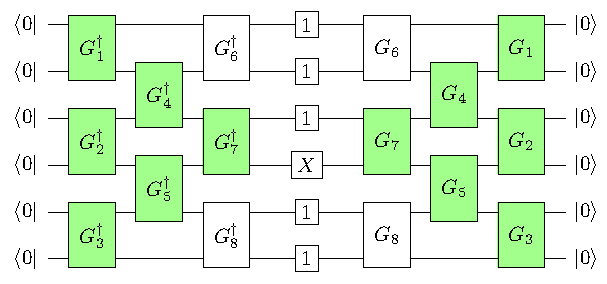
\includegraphics[width=0.8\textwidth]{figures/figures_tex/causalcone.pdf}
    \caption{A causal cone of a Pauli string. Highlighted gates do not cancel in $U^\dagger h U$, where $U$ is the quantum circuit pictured. Reprinted from \cite{uvarov_barren_2021}.}
    \label{fig:causal_cone}
\end{figure}{}

\begin{definition}[Mixer]

    Let $\mc{Y}$ be a subset of the qubit registry. Define the \textit{local mixing operator}, or simply a \textit{mixer}\footnote{The mixer is in fact a quantum channel since it is defined by its own Kraus decomposition.}  $M_{\mc{Y}}: \operatorname{End} (\mc{H}\otimes \mc{H}) \rightarrow \operatorname{End} (\mc{H}\otimes \mc{H})$ as follows:
    \begin{equation}
    \begin{aligned}
        \label{eq:m2}
        & M_{ \mc{Y}} (h_1 \otimes h_2) = \int d\mu_{\mc{Y}} (U)
        (U^\dagger \otimes U^\dagger)
        (h_1 \otimes h_2)
        (U \otimes U),
    \end{aligned}{}
    \end{equation}{}
    where $\mu_{\mc{Y}}$ is a Haar distribution of unitaries acting nontrivially on $\mc{Y}$ and trivially on all other qubits.
    
\end{definition}


\begin{proposition}
    \label{prop:m2_decomposed}
    Let $h$ be a Pauli string. If its substring $h_{\mc{Y}}$ is nontrivial, then
    
    \begin{equation}
        M_{\mc{Y}}(h \otimes h) = \frac{1}{4^{|\mc{Y}|} - 1} \left( \sum_{\sigma_\mc{Y} \neq \mathbbm{1}} (\sigma_{\mc{Y}} \otimes h_{\mc{H} \setminus \mc{Y}})^{\otimes 2}\right),
    \end{equation}{}
    where the summation extends over all nontrivial Pauli substrings $\sigma_{\mc{Y}}$.
    Otherwise,  $M_{\mc{Y}}(h \otimes h) = h \otimes h$.
    
\end{proposition}{}

\begin{proof}
    We first apply formula (\ref{eq:haar_integral_2}):
    \begin{equation}
        % M_{\mc{Y}}(h \otimes h) = \frac{1}{4^{|\mc{Y}|} - 1} 
        % (h \otimes h)_{\mc{H} \setminus \mc{Y}} \left[ \left( \Tr  (h \otimes h)_{\mc{Y}} \right) (\mathbbm{1} \otimes \mathbbm{1})_{\mc{Y}}
        % \right]
    \begin{aligned}
    \label{eq:m2_proof_1}
        & M_{\mc{Y}}(h \otimes h) = \\
        & = \frac{1}{4^{|\mc{Y}|} - 1} (h \otimes h)_{\mc{H} \setminus \mc{Y}} \otimes \left[  
        \left(\Tr (h \otimes h)_{\mc{Y}}  - \frac{1}{2^{|\mc{Y}|}} \Tr \mc{S}_{\mc{Y}} (h \otimes h)_{\mc{Y}} \right) \mathbbm{1} \otimes  \mathbbm{1} + \right. \\
        & \left. + \left(\Tr \mc{S}_{\mc{Y}} (h \otimes h)_{\mc{Y}}  - \frac{1}{2^{|\mc{Y}|}} \Tr (h \otimes h)_{\mc{Y}}\right) \mc{S}_\mc{Y} \right],
    \end{aligned}{} 
    \end{equation}
    where $\mc{S}_\mc{Y}$ is the swap operator permuting pairs of qubits $(i, i')$ for $i \in \mc{Y}$. It means that $\mc{S}_\mc{Y}$ is a tensor product of two-qubit swap gates $\mc{S}_2$. 
    First, note that $\Tr \mc{S}_{\mc{Y}} (h \otimes h)_{\mc{Y}} = 2^{|\mc{Y}|}$ and $\Tr (h \otimes h)_{\mc{Y}}$ is equal to zero for nontrivial $h_\mc{Y}$ and $4^{|\mc{Y}|}$ for a trivial substring. Next, $\mathcal{S}_2$ is decomposed as 
    \begin{equation}
    \label{eq:swap_decomp}
        \mathcal{S}_2 = \frac{1}{2}\left(X \otimes X + Y \otimes Y + Z \otimes Z + \mathbbm{1} \otimes \mathbbm{1} \right).
    \end{equation}
    Applying this decomposition to $\mc{S}_\mc{Y}$ yields a sum of all possible super Pauli strings (including the trivial string):
    \begin{equation}
        \mc{S}_{\mc{Y}} = \frac{1}{2^\mc{|Y|}} \sum_{\sigma_1, ..., \sigma_\mc{|Y|}}
        (\sigma_1 \otimes \sigma_2 \otimes ... \otimes \sigma_\mc{|Y|})^{\otimes 2}.
    \end{equation}
    Substituting this decomposition into \eqref{eq:m2_proof_1} we recover the desired result.
\end{proof}{}

This means that, after application of the local mixer channel $M_\mc{Y}$ to a super Pauli string $h \otimes h$, we forget the exact Pauli operators in the registry $\mc{Y}$, and replace them will a uniform linear combination of all possible nontrivial Pauli strings.For example, consider a single-qubit mixing channel $M_2$ acting on qubits $(2, 2')$.
Then $M_2 ((XX)^{\otimes 2}) = \frac{1}{3} ( (XX)^{\otimes 2} + (XY)^{\otimes 2} + (XZ)^{\otimes 2})$. On the contrary, a string $(XI)^{\otimes 2}$ will be invariant under the mixing channel: $M_2 ((XI)^{\otimes 2}) = (XI)^{\otimes 2}$.

Importantly, mixer channels do not accept Pauli strings of the type $h_1 \otimes h_2$, where $h_1 \neq h_2$. The following statement can also be proven by application of formula (\ref{eq:haar_integral_2}).

\begin{proposition}
    \label{prop:mixer_kills_asymmetry}
    Let $h_1, h_2$ be Pauli strings such that their restriction on a registry $\mc{Y}$ is different. Then $\mc{M_Y} (h_1 \otimes h_2) = 0$.
\end{proposition}


\subsubsection{Action of many mixer channels}

When we consider a circuit made of many blocks, we essentially model them with a sequence of local mixers. 

\begin{proposition}
    \label{prop:paulis_decouple}
    Let $\mc{Y}_1, ..., \mc{Y}_N$ be a collection of qubit subsets
    such that $\mc{Y}_1 \cup ... \cup \mc{Y}_N$ contains all $n$ qubits (the subsets are allowed to intersect). Let $h_1, h_2$ be two distinct Pauli strings. Then, 
    $M_{ \mc{Y}_N} \circ \dots \circ  M_{ \mc{Y}_1} (h_1 \otimes h_2) = 0.$
\end{proposition}{}
\begin{proof}
    Let the strings be different in position $k$. If $k \notin \mc{Y}_j$, then $M_{ \mc{Y}_j}$ will output a sum of Pauli strings $h_{1, j} \otimes h_{2, j}$ that still have different entries in positions $k$ and $k'$. If $k \in \mc{Y}_j$, the output will be zero by virtue of Proposition~\ref{prop:mixer_kills_asymmetry}. Since every qubit is contained in the support of some mixer, the latter must happen for some $j$.
\end{proof}

\begin{remark}
    The sum of coefficients of the Pauli strings is conserved by the mixers. However, suppose that the mixers act on all qubits in the support of some nontrivial Pauli string $h$, with $C$ being support the causal cone of $h$ under the mixers. After the action of the mixers, $h \otimes h$ is replaced by the sum of all possible super Pauli strings that are nontrivial on $|C|$ trivial on the complement $[n] \backslash |C|$, with the weights equal to $(4^{-|C|} - 1)$.
\end{remark}


\subsubsection{Commutator operator}

Equation (\ref{eq:varde_integral}) contains an expression depending on $([\rmi F, U^\dagger H U])^{\otimes 2}$ for some $U$, $H$, and $F$. For convenience we introduce a commutator operator $\mc{C}_{F} \in \operatorname{End}(\mc{H} \otimes \mc{H})  \rightarrow \operatorname{End}(\mc{H} \otimes \mc{H})$, which maps $A \otimes B$ to $[\rmi F, A] \otimes [\rmi F, B]$. Unlike the mixer operator, $\mc{C}_F$ is no longer a quantum channel since it does not preserve trace. Nonetheless, it is important for our purposes to consider its action on Pauli strings. We will henceforth assume that $F$ is a Pauli string. Graphically, we can express this superoperator like this:
% (see Fig. \ref{fig:mixer_and_commut}). 

\newcommand{\legw}{1}
\newcommand{\gapw}{2}
\newcommand{\gaph}{1}
\newcommand{\barh}{0.6}
\newcommand{\wireh}{0.2}
\newcommand{\wiregap}{0.5}
\newcommand{\wirel}{0.3}

\begin{equation}
    \mc{C}_F(\star) =
    \adjustbox{raise=-7pt}{
    \begin{tikzpicture}[thick,scale=0.5]
    \node[blank] at (\gapw/2 + \legw, \gaph/2) {$\star$};
    
    
    \draw 
    (0, 0) 
    -- (0, \gaph + \barh) 
    -- (\gapw + \legw + \legw,\gaph + \barh)
    -- (\gapw + \legw + \legw,0)
    -- (\gapw + \legw,0)
    -- (\gapw + \legw, \gaph)
    -- (\legw, \gaph)
    -- (\legw,0)
    -- (0, 0)
    
    (0, \wireh) -- (-\wirel, \wireh)
    (0, \wireh + \wiregap) -- (-\wirel, \wireh + \wiregap)
    
    (\legw, \wireh) -- (\legw + \wirel, \wireh)
    (\legw, \wireh + \wiregap) -- (\legw + \wirel, \wireh + \wiregap)
    
    (\legw + \gapw, \wireh) -- (\legw + \gapw - \wirel, \wireh)
    (\legw + \gapw, \wireh + \wiregap) -- (\legw + \gapw - \wirel, \wireh + \wiregap)
    
    (\gapw + \legw + \legw, \wireh) -- (\gapw + \legw + \legw + \wirel, \wireh)
    (\gapw + \legw + \legw, \wireh + \wiregap) -- (\gapw + \legw + \legw + \wirel, \wireh + \wiregap)
    
    ;
    \end{tikzpicture}
    }
\end{equation}

Unlike the mixer, $\mc{C}_{F}$ does not care if the Pauli strings in the tensor copies of $\operatorname{End}(\mc{H})$ are identical: $[\rmi F, A] \otimes [\rmi F, B]$ does not necessarily vanish for distinct $A, B$.

Any two Pauli strings either commute or anticommute with each other. Let $\boldsymbol{\sigma}_1$ and $\boldsymbol{\sigma}_2$ be Pauli strings on $\mc{H}$. Then $\mc{C}_F (\boldsymbol{\sigma}_1 \otimes \boldsymbol{\sigma}_2)$ does not vanish if and only if both $\boldsymbol{\sigma}_1$ and $\boldsymbol{\sigma}_2$ anticommute with $F$. 
% In which case, $\mc{C}_F (\boldsymbol{\sigma}_1 \otimes \boldsymbol{\sigma}_2) = 4 (\boldsymbol{\eta}_1 \otimes \boldsymbol{\eta}_2)$ for some Pauli strings $\boldsymbol{\eta}_1, \boldsymbol{\eta}_2$.
A product of two Pauli strings is again a Pauli string, possibly multiplied by a power of $\rmi$. An operator $[\rmi F, \boldsymbol{\sigma}]$ is Hermitian and proportional to a Pauli string, so it is equal to $\pm 2 \boldsymbol{\eta}$ for some Pauli string $\boldsymbol{\eta}$. A remarkable property of $\mc{C}_F$ is that for super Pauli strings $\boldsymbol{\sigma} \otimes \boldsymbol{\sigma}$ such that $F$ anticommutes with $\boldsymbol{\sigma}$, the sign is canceled, so $\mc{C}_F(\boldsymbol{\sigma} \otimes \boldsymbol{\sigma}) = 4 \boldsymbol{\eta} \otimes \boldsymbol{\eta}$ for some $\boldsymbol{\eta}$.

We can now consider what happens when there are mixers before and after $\mc{C}_F$.

% $F \boldsymbol{\sigma}_1 = (-1)^{a} \boldsymbol{\sigma}_1 \boldsymbol{\sigma}_iF , F\boldsymbol{\sigma}_2 = (-1)^b \boldsymbol{\sigma}_2 F$.

\begin{proposition}
    \label{prop:commutator_old}
    The following identities hold:
    \begin{enumerate}
        \item For every $F \in \mathrm{Herm}(\mc{Y})$, $\mc{C}_{F}(\id_{\mc{Y}} \otimes \id_{\mc{Y}})$ vanishes. Thus, $M_{\mc{Y}} \circ \mc{C}_F \circ M_{\mc{Y}} (\id_{\mc{Y}} \otimes \id_{\mc{Y}})=0$.
        \item Let $F$ be a nontrivial Pauli string acting on $\mc{Y}$. Then, for any nontrivial Pauli string $h$ acting on $\mc{Y}$
        \begin{equation}
            \label{eq:sandwiched_commutator}
             M_{\mc{Y}} \circ \mc{C}_{F} \circ M_{\mc{Y}} \left( h^{\otimes 2}\right) = \frac{2 \cdot 4^{|\mc{Y}|}}{4^{|\mc{Y}|} - 1} M\left( h^{\otimes 2}\right).
        \end{equation}
    \end{enumerate}{}
\end{proposition}{}
    
\begin{proof}
    The first part follows directly: identity operator commutes with any other operator.
    % \textcolor{blue}{\textbf{[In my opinion, this is clearer than ``identity operator is central'' --- Alexey]}} 
    To prove the second part, we will sequentially apply the operators in the left-hand side of \eqref{eq:sandwiched_commutator}. First, the local mixing operator returns a linear combination of all nontrivial Pauli strings $\boldsymbol{\sigma}_i$: $M_{\mc{Y}} \left( h^{\otimes 2}\right) = 1/ (4^{|\mc{Y}|} - 1)\sum \boldsymbol{\sigma}_i^{\otimes 2}$. After applying $\mc{C}_{\mc{Y}}$ to each super Pauli string we either get zero for those commuting with $F$ and some other super Pauli string $\boldsymbol{\kappa}_i \otimes \boldsymbol{\kappa}_i$ multiplied by 4 for those anticommuting with $F$:
    \begin{equation}
        ([\rmi F, \boldsymbol{\sigma}_i])^{\otimes 2} = (\pm 2 \boldsymbol{\kappa}_i)^{\otimes 2} = 4 \boldsymbol{\kappa}_i^{\otimes 2}.
    \end{equation}

    For any nontrivial Pauli string $F$, there are exactly $4^{|\mc{Y}|} / 2$ nontrivial Pauli strings that anticommute with $F$. 
    Indeed, let $F$ contain $m$ nontrivial Pauli matrices and let $P$ be some Pauli string that we wish to construct, so that it anticommutes with $F$. How many ways of constructing $P$ are there? There must be an odd number of sites $j$ such that Pauli matrices $F_j$ and $P_j$ are both nontrivial and not equal to each other. We can pick such sites in $2^{m - 1}$ ways. Then, for each of these sites, there is a choice of 2 Pauli matrices not commuting with $F_j$. For all sites where $F_j$ is nontrivial, but which are not included in our selection, $P_j$ is either equal to $\id$ or to $F_j$. Finally, in all sites where $F_k = \id$, we are free to choose any Pauli matrix. Hence, when the choice of sites is fixed, we have $2^m 4^{|\mc{Y}| - m}$ options. Multiplying this by $2^{m - 1}$, we get $4^{|\mc{Y}|} / 2$.
    
    Overall, the result is the following: the first mixer produces a sum of all possible nontrivial super Pauli strings, the commutator $\mc{C}$ keeps $4^{|\mc{Y}|} / 2$ of them and multiplies them by 4, and then the second mixer again turns each super string into a sum of all possible super Pauli strings. Collecting the prefactors yields \eqref{eq:sandwiched_commutator}.
    
    
\end{proof}








\subsection{Main statement}

Now we are ready to formulate the main result of this section \cite{uvarov_barren_2021}:

\begin{theorem}
    \label{thm:block_plateaus}
    Let $H$ be an $n$-qubit Hamiltonian consisting of Pauli strings $h_i$: $H = \sum c_i h_i$ with finite $c_i \in \mathbb{R}$. Let the ansatz $U$ consist of $l$ layers, and denote $l_c$ the layer which contains the block $G_k$ depending on parameter $\theta_a$. 
    % \textcolor{blue}{\textbf{[I don't think we should write $\theta_k$; a block typically depends on more than one parameter. Maybe we can highlight its special role in some other way, like $\tilde{\theta}$ or $\hat{\theta}$? --- Alexey]}}. 
    Let each block of the ansatz be an independently parametrized local 2-design. Let the block $G$ also be decomposable into $G = G_A e^{-i \theta_a F} G_B$, where $G_A$ and $G_B$ are local 2-designs not depending on $\theta_a$. Then, the variance of the gradient of $E$ with respect to that parameter is bounded below as follows:
    
    \begin{equation}
        \operatorname{Var} \partial_a E \geq \frac{2 \cdot 4^{|\mc{Y}_k|}}{4^{|\mc{Y}_k|} - 1} \left( \frac34 \right)^{l - l_c}  \sum_i c_i^2 \cdot 3^{-|C(h_i, U)|},
    \end{equation}{}
    where $|C(h_j, U)|$ is the number of qubits in the causal cone of the $j^{th}$ Pauli string, and the summation is over those Pauli strings whose causal cone contains the block $G$.
\end{theorem}{}

The proof of this theorem uses the fact that $\partial_a E (h_i)$ are uncorrelated random variables:

\begin{proposition}
\label{lemma:expectations_decouple}
In the conditions of Theorem \ref{thm:block_plateaus}, the individual Pauli string coefficients make independent contributions to the total variance:
\begin{equation}
    \operatorname{Var} \partial_a E (H) = \sum_i c_i^2 \operatorname{Var} \partial_a E (h_i).
\end{equation}
\end{proposition}



\subsection{Idea of the proof}

The proof is conceptually not difficult, but quite laborious. To estimate the variance, we will need to integrate $(\partial_aE) ^2$ over all possible assignments of the parameters $\boldsymbol{\theta}$. Since we assumed that the blocks are parametrized independently, we can also take their expected values independently. If $U_p$ depends on parameters $\boldsymbol{\theta}_j =  \theta_{j_1}, ..., \theta_{j_m}$ for some $j_1, ..., j_m$, then the operator we care about takes the following form:

%%%%%% The usage of \adjustbox is not elegant, but I don't care
\begin{equation}
\label{eq:true_mixer}
M = \int (U_p^\dagger \otimes U_p^\dagger) (\star) (U_p \otimes U_p) 
\mathrm{d} \boldsymbol{\theta}_j
= \int 
% \includegraphics[valign=m,width=0.1\linewidth]
% {
\adjustbox{raise=31pt}{
\Qcircuit @C=1em @R=.7em 
{& \multigate{1}{U^\dagger} &  \multigate{3}{\star} 
& \multigate{1}{U} & \qw
\\
& \ghost{U^\dagger} & \ghost{\star}
& \ghost{U} & \qw
\\
& \multigate{1}{U^\dagger} & \ghost{\star}
& \multigate{1}{U} & \qw
\\
& \ghost{U^\dagger} & \ghost{\star}
& \ghost{U} & \qw
}
}
\mathrm{d} \boldsymbol{\theta}_j
\end{equation}
where the star ($\star$) is a placeholder for a Hermitian operator on $\mc{H} \otimes \mc{H}$. The commutator found in \eqref{eq:partial_E} can also be viewed as a superoperator $[\rmi F, \star]^{\otimes 2}$. 

In this graphical language, the value of $\operatorname{Var} \partial_a E$ is expressed as a diagram shown in Fig.~\ref{fig:variance_as_diagram}.

Instead of evaluating the action of operators like $M$ for a specific ansatz, we instead assume that each block of the ansatz constitutes a local 2-design, in which case one can compute their action exactly. We will refer to such operators as ``mixing operators''.

The action $[\rmi F, \star]^{\otimes 2}$ can be written down explicitly using the assumption that there are two mixing operators around it. In which case, its role reduces to eliminating those Pauli strings that don't share support with $F$, and multiplying all other strings by a constant. We estimate the number of strings that survive this operation by tracing a path along the structure of the ansatz.

After all these operators, we end up with a number of Pauli strings with some coefficients. Taking the expectation w.r.t.\ the zero kets eliminates those strings that contain $X$ or $Y$ Pauli matrices. We estimate the share of Pauli strings that are not eliminated in the process. The sum of their coefficients is the final value that we are after.

\begin{figure}
    % \centering
    \begin{tikzpicture}
    \node[] (formula) {$\operatorname{Var} \partial_a E = \displaystyle{\int} \mathrm{d} \boldsymbol{\theta}$};
    \node (fig1) [above right of =formula, xshift=7cm, yshift=1cm] {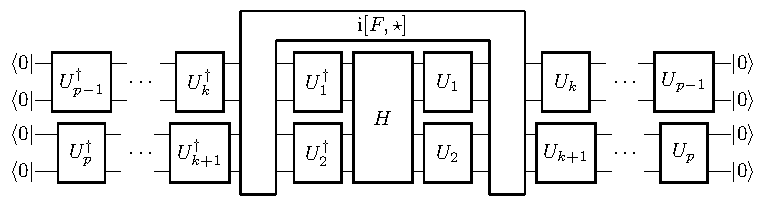
\includegraphics[width=0.7\linewidth]{figures/vardE.pdf}};
    \node (fig2) [below right of =formula, xshift=7cm, yshift=-0.6cm] {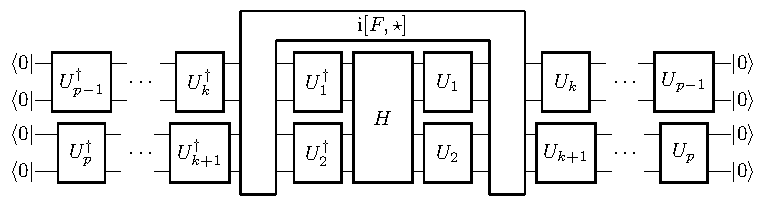
\includegraphics[width=0.7\linewidth]{figures/vardE.pdf}};
    \end{tikzpicture}
    
    
    % \includegraphics[width=\linewidth]{variance_as_diagram.jpg}
    \caption{Variance of the derivative of $E$, expressed as an integration over all possible assignments of $\boldsymbol{\theta}$. Reprinted from~\cite{uvarov_barren_2021}.
    % Each triangle denotes a zero ket vector $\ket{0}$.
    }
    \label{fig:variance_as_diagram}
\end{figure}

In the following sections, we will first derive the necessary properties of the mixing operators and of the commutator-induced superoperator. Then we will use them to prove the main statement.

\subsection{Proof of the main statement}

Following the definitions, the variance can be expressed as an average of a certain operator over the zero ket vectors 
$\ket{\boldsymbol{00}} = (\ket{\boldsymbol{0}} \otimes \ket{\boldsymbol{0}})$. To write down that operator, we use the assumption that individual blocks $G_1, ..., G_q$ are local 2-designs, and replace the integration with local mixing operators $M_{\mc{Y}_1} ... M_{\mc{Y}_q}$:
\begin{equation}
\label{eq:all_mixers}
\Var \partial_a E (H) 
= \bra{\boldsymbol{00}}
M_{ \mc{Y}_1} \circ 
\dots \circ  M_{ \mc{Y}_k} \circ \mc{C} \circ M_{ \mc{Y}_k} \circ 
\dots \circ  M_{ \mc{Y}_q} (H \otimes H) \ket{\boldsymbol{00}}.
\end{equation}{}
Note the reverse order of the mixing operators: if the ansatz state is $\ket{\psi} = G_q ... G_1 \ket{\mathbf{0}}$, then $\bra{\psi} H \ket{\psi} = 
\bra{\mathbf{0}} G_1^\dagger ... G_q^\dagger H G_q ... G_1 \ket{\mathbf{0}}$. 
Therefore, in the Heisenberg picture, the conjugation with unitaries reverses.

The action of all operators in the right hand side of \eqref{eq:all_mixers}
is linear, so we can replace $H \otimes H$ by $\sum_{i, j}c_i c_j h_i \otimes h_j$. From Proposition \ref{prop:paulis_decouple} we know that all terms with $i \neq j$ will vanish, so we arrive at
\begin{equation}
    \label{eq:paulis_decouple}
    \Var \partial_a E (H) = \sum_i c_i^2 \Var \partial_a E (h_i),
\end{equation}
effectively reducing the problem to the case when the Hamiltonian of interest is a single Pauli string $h$.

In the next three subsections, we estimate the value of $\Var \partial_a E (H)$ by sequentially applying the superoperators shown in \eqref{eq:all_mixers}.

\subsubsection{First portion of mixing operators}

Let us now follow the evolution of some Pauli string $h_i$ along the application of the mixing operators before the commutation operator $\mc{C}$. Each mixing operator replaces the super Pauli string with the sum of super Pauli strings with all possible nontrivial substrings in its support. For example, a two qubit mixing operator takes one super Pauli string and returns 15 super Pauli strings (see Proposition \ref{prop:m2_decomposed}):

\begin{equation}
    M\left((X \otimes X)^{\otimes 2} \right) = \frac{1}{15}
    \left( \sum_{i,j} (\sigma_i \otimes \sigma_j)^{\otimes 2}
    + \sum_{i} \left((\sigma_i \otimes \mathbbm{1})^{\otimes 2}
    + (\mathbbm{1} \otimes \sigma_i)^{\otimes 2} \right)
    \right).
\end{equation}

After a sequence of such mixing operators, the super Pauli string $h \otimes h$ is transformed into a sum of some other super Pauli strings $g_\alpha$: $M_{\mc{Y}_k} \circ ... \circ M_{\mc{Y}_q} (h_i \otimes h_i) = \sum c'_\alpha g_\alpha \otimes g_\alpha$. This collection is rather difficult to describe, however, from the properties of the mixers we know that (i) the coefficients $c'_\alpha$ sum up to one, and that (ii) the support of every Pauli string $g_\alpha$ is bounded by the support of the causal cone $|C(h, U)|$. Also, one can show that every qubit in the causal cone is in the support of some Pauli string $g_\alpha$.

\subsubsection{Elimination of terms by commutator}

The block $G_k$ corresponds to a triple of operators $M_{ \mc{Y}_k} \circ \mc{C} \circ M_{ \mc{Y}_k}$, of which we already used the first one. The pair of operators $M_{\mc{Y}_k} \mc{C}$ now acts in the following way: the strings whose support does not intersect that of $\mc{C}$ are eliminated, while all other strings are multiplied by a constant coefficient depending on the size of the block containing $\mc{C}$ (see Proposition \ref{prop:commutator_old}). To bound the number of surviving terms from below, we explicitly track a subset of such terms. 
% We need to estimate how many terms survive after the commutator. Let the block with the commutator be situated in the layer number $L_c$. 

If the block $G_k$ is outside the causal cone of $h \otimes h$, then the derivative $\partial_\theta E$ is trivially zero. 
% \out{applying the commutator necessarily yields zero, as tuning the corresponding gate does not change $U^\dagger h U$.}
So, excluding this case, let us assume that the block $G_k$ is within the causal cone of $h$. This means that we can find a sequence of blocks $G_{j_l}, ... G_{j_{l_c + 1}}$ situated in layers $l, ..., l_c + 1$, such that the first one shares support with $h$, and each $G_{j_{k-1}}$ shares support with $G_{j_k}$. Finally, we require that $G_{j_{l_c + 1}}$ shares support with the block $G_k$. Thus, we have established a causal path from $h$ to the commutator (see Fig. \ref{fig:comm_path}). 

Now, the output of the mixer $M_{j_l}$ contains $4^{|\mc{Y}_{j_l}|} - 1$ super Pauli strings with equal coefficients, at least $3/4$ of which act nontrivially in the support of $G_{j_{l-1}}$. For example, if $G_{j_l}$ is a two-qubit block, it outputs 15 super Pauli strings, of which 12 share support with the next block $G_{j_{l - 1}}$. The next mixer 
$M_{j_{l - 1}}$ takes those super Pauli strings, and for each of them, outputs $4^{|\mc{Y}_{j_{l - 1}}|} - 1$ super Pauli strings, of which at least $3/4$ again have nontrivial action in the support of the next block. Continuing on, we find that the total weight of such super Pauli strings is at least $(3/4)^{l - l_c}$. Then it gets multiplied by $\frac{2 \cdot 4^{|\mc{Y}_k|}}{4^{|\mc{Y}_k|} - 1}$. 
% which is always greater than 2, so the estimate we end up with is $2 \cdot (3/4)^{l - l_c}$.


Note that the blocks outside the specified path can increase this number, but not decrease it. For example, in the notation of Fig. \ref{fig:comm_path}, we first acted with the mixer $M_{10}$, corresponding to the block $G_{10}$, and got a collection of super Pauli strings in the output, some of which act nontrivially on qubits 3 and 4, the support of $G_8$. The action of the mixer $M_{11}$ cannot make those strings lose the nontrivial action on that support. In principle, such block could bring more strings to act nontrivially there, but for a lower bound this is not important.

\begin{figure}
    %% Another figure with hacky tricks
    %% https://tex.stackexchange.com/questions/389588/
    \centering
    % \includegraphics[width=\linewidth]{commutator_path.jpg}
    \begin{pgfpicture}{0em}{0em}{0em}{0em}
    \color{gray!70}
    \pgfrect[fill]{\pgfpoint{11.32em}{-4.25em}}{\pgfpoint{2.65em}{2.8em}}
    \pgfrect[fill]{\pgfpoint{8.1em}{-6.15em}}{\pgfpoint{2.25em}{2.8em}}
    \pgfrect[fill]{\pgfpoint{4.9em}{-8.05em}}{\pgfpoint{2.2em}{2.8em}}
    \color{green!80!yellow!45!white}
    \pgfrect[fill]{\pgfpoint{1.65em}{-6.15em}}{\pgfpoint{2.25em}{2.8em}}
    % \pgfgrid[stepx=0.2em, stepy=0.2em]{\pgfpoint{1.65em}{-6.15em}}{\pgfpoint{3.9em}{-3.35em}}
    \end{pgfpicture}
    \mbox{
            \Qcircuit @C=1.0em @R=1.0em {
            \lstick{\ket{0}} 
            & \multigate{1}{G_1} 
            & \qw 
            & \multigate{1}{G_7}    
            & \qw 
            & \qw
            & \rstick{1}
            \\
            \lstick{\ket{0}} 
            & \ghost{G_1} 
            & \multigate{1}{G_4} 
            & \ghost{G_7} 
            & \multigate{1}{G_{10}} 
            & \qw  
            & \rstick{1}
            \\
            \lstick{\ket{0}} 
            & \multigate{1}{G_2}  
            & \ghost{G_4}
            & \multigate{1}{G_8} 
            & \ghost{G_{10}}
            & \qw  
            & \rstick{X}
            \\
            \lstick{\ket{0}} 
            & \ghost{G_2} 
            & \multigate{1}{G_5} 
            & \ghost{G_8}
            & \multigate{1}{G_{11}} 
            & \qw  
            & \rstick{X}
            \\
            \lstick{\ket{0}} 
            & \multigate{1}{G_3}
            & \ghost{G_5} 
            & \multigate{1}{G_9}
            & \ghost{G_{11}} 
            & \qw  
            & \rstick{1}
            \\
            \lstick{\ket{0}} 
            & \ghost{G_3} 
            & \multigate{1}{G_6}
            & \ghost{G_8}
            & \multigate{1}{G_{12}}
            & \qw
            & \rstick{1}
            \\
            \lstick{\ket{0}} 
            & \qw
            & \ghost{G_6}
            & \qw
            & \ghost{G_{12}}
            & \qw
            & \rstick{1}
            \\
              }
        }
    \caption{An example of a path constructed out of blocks with nontrivial inputs. Dark blocks correspond to mixing operators, highlighted block contains the commutator.}
    \label{fig:comm_path}
\end{figure}{}

\subsubsection{Second portion of the mixing operators}

Let us apply all the remaining operators except the set of mixers $B = \{ M_{\mc{Y}_{1}}, ..., M_{\mc{Y}_m} \}$ corresponding to the first layer of the ansatz. Upon doing that, we get a linear combination of super Pauli strings $\sum_\alpha c''_\alpha g'_\alpha \otimes  g'_\alpha$. The coefficients $c''_\alpha$ sum up to at least $\frac{2 \cdot 4^{|\mc{Y}_k|}}{4^{|\mc{Y}_k|} - 1} \cdot (3/4)^{l - l_c} $. Each super string $g'_\alpha \otimes  g'_\alpha$ will then go through this layer of mixers and then the output will get averaged over the zero ket vector $\ket{\boldsymbol{00}}$.

For every $g'_\alpha \otimes  g'_\alpha$, the number resulting from this series of operations is greater or equal to $\prod_{M_{\mc{Y}} \in B} \frac{2^{|\mc{Y}|} - 1}{4^{|\mc{Y}|} - 1}$. The super Pauli string $g'_\alpha \otimes  g'_\alpha$ can act trivially or nontrivially on the support of each $M_{\mc{Y}} \in B$. If it acts trivially, then $M_{\mc{Y}}$ does nothing. In the opposite case, $M_{\mc{Y}}$ yields $4^{|\mc{Y}|} - 1$ super Pauli strings with equal weights. Of these strings, only $2^{|\mc{Y}|} - 1$ consist entirely of identity matrices and Pauli $Z$ matrices, and only these strings yield a 1 when averaged over $\ket{\boldsymbol{00}}$. Repeating for all mixers in $B$ yields the lower bound $\prod_{M_{\mc{Y}} \in B} \frac{2^{|\mc{Y}|} - 1}{4^{|\mc{Y}|} - 1}$.

Summing up all of the above, we write the lower bound on $\Var \partial_\theta E(h_i)$:
\begin{equation}
\label{eq:var_theta}
    \partial_\theta E (h) \geq \frac{2 \cdot 4^{|\mc{Y}_k|}}{4^{|\mc{Y}_k|} - 1} \left( \frac34 \right)^{l - l_c} 
    \prod_{M_{\mc{Y}} \in B} 
    \frac{2^{|\mc{Y}|} - 1}{4^{|\mc{Y}|} - 1} = 
    \frac{2 \cdot 4^{|\mc{Y}_k|}}{4^{|\mc{Y}_k|} - 1} \left( \frac34 \right)^{l - l_c}
    \prod_{M_{\mc{Y}} \in B} 
    \frac{1}{2^{|\mc{Y}|} + 1}.
\end{equation}{}
% where $B$ is the set of operators in the first layer of the causal cone of $h_i$ and provided that block with parameter $\theta$ is inside the causal cone.

The last product can be bounded from below by $3^{-|C(h, U)|}$. Here is how: $1/ (2^{|\mc{Y}|} + 1) = (1/2^{|\mc{Y}|}) \cdot 1/(1 + 2^{-|\mc{Y}|})$. Since $|\mc{Y}| \geq 1$, then the second factor of the right-hand side of this equality is greater or equal than $2/3$. The product can be then transformed as follows:


\begin{equation}
\label{eq:massage_var_theta}
     \prod_{M_{\mc{Y}} \in B} 
    \frac{1}{2^{|\mc{Y}|} + 1} \geq      
    \prod_{M_{\mc{Y}} \in B}  \frac{1}{2^{|\mc{Y}|}} \frac{2}{3}
    = \left( \frac{2}{3} \right)^{|B|} \frac{1}{2^{|C(h, U)|}}.
\end{equation}{}
Now observe that the number of blocks is not greater than the number of qubits, and hence the last part of \eqref{eq:massage_var_theta} is lower bounded by $3^{-|C(h, U)|}$, which concludes the proof.

\subsection{Extension of the theorem}

In the formulation of Theorem~\ref{thm:block_plateaus}, we required that the partial blocks $G_A$, $G_B$ form 2-designs themselves. This assumption can be partially relieved. We know from Proposition~\ref{prop:ad_is_pauli_orthogonal} that $\mathrm{Ad}_{G_B \otimes G_B}$ preserves the 2-norm of its input. This means that the 1-norm --- the quantity preserved by the mixers --- will be multiplied by a factor in $[4^{-|\mc{Y}|}, 4^{|\mc{Y}|}]$ due to the equivalence of vector norms. The precise composition of its output does not matter: the subsequent mixer operators will essentially erase it, only caring about the causal cone structure. Therefore, we can remove the requirement that $G_B$ forms a 2-design at the cost of a $\Theta(1)$ multiple to the lower bound.

Removing the requirement that $G_A$ is a 2-design is more difficult. Suppose that just before $G_A$ we have some sum of super Pauli strings $\sum_\sigma \tilde{c}_\sigma \sigma \otimes \sigma$. If $G_A$ is a 2-design, we can reason about the proportion of terms that will end up anticommuting with $F$. For arbitrary $G_A$, the worst case it that all terms $\textrm{Ad}_{G_A} (\sigma)$ commute with $F$, causing the overall variance to go to zero. To rule out this scenario, one will have to understand the distribution of coefficients $\tilde{c}_\sigma$.





\section{Numerical results}

\subsection{Proximity of local blocks to 2-designs}
\label{subsec:proximity_to_designs}

It is known that approximate 2-designs can be prepared by a polynomial depth random circuit \cite{harrow_approximate_2018,brandao_local_2016}. However, here we are interested in local blocks whose properties are not guaranteed by asymptotic estimates.

We performed a series of numerical experiments to compare certain two-qubit blocks to exact unitary designs. A simple way of evaluating the proximity of the gate families to the Haar measure is to measure the distance to the so-called quantum $t$-tensor product expander (TPE) \cite{brandao_local_2016,low_pseudo-randomness_2010}. A family of random unitary gates $\nu$ is a $\lambda$-approximate TPE if $||\mathbb{E}_{Haar} (U^{\otimes t} \otimes (U^*)^{\otimes t}) - \mathbb{E}_\nu (U^{\otimes t} \otimes (U^*)^{\otimes t}) ||_p \leq \lambda$ for $p=\infty$. 
The trace definition of an approximate $t$-design involves the same quantity for $p = 1$. 

Finally, for $p=2$ this quantity can be related to the coefficients of Pauli decomposition of a Hamiltonian going through a mixing operator.  Let $H = \sum c_i \sigma_i$ be a Hamiltonian on $n$ qubits. Recall that Pauli strings form an orthogonal basis. Since the Hilbert-Schmidt inner product is the same as the scalar product of matrices as vectors in $\mathbb{R}^{2^n \times 2^n}$, this also applies to their reshaping to vectors. Then one can verify that $||\mathrm{vec}(H)||_2 = 
2^{\frac{n}{2}} \sqrt{\sum_i |c_i|^2}
\equiv ||\mathbf{c}||_2 \cdot 2^{\frac{n}{2}}$. This works when $\sigma_i$ are super Pauli strings. The operator 2-norm of $\mathbb{E}_{Haar} (U^{\otimes t} \otimes (U^*)^{\otimes t}) - \mathbb{E}_{\mu} (U^{\otimes t} \otimes (U^*)^{\otimes t})$, provides an upper bound on the vector norm of the output of this operator, meaning that this is the maximum norm of the discrepancy from the perfect output for an input of unit norm. For a super Pauli string $h \otimes h$, this error $\lambda_2$ upper bounds the 2-norm of the vector $(\mathbf{c} - \mathbf{c}_{\text{Haar}})$.

We will denote the aforementioned $p$-norms as $\lambda_1$, $\lambda_2$ and $\lambda_\infty$. 

\begin{table}
    \centering
    \begin{tabularx}{\textwidth}{|>{\centering}X|c|c|c|c|}
    \hline
        Block & Circuit diagram or matrix & $\lambda_1$ & $\lambda_\infty$ & $\lambda_2$\\
        \hline
        $X$, $Z$, and $ZZ$ rotations &  
        % \mbox{
            $\Qcircuit @C=1.0em @R=1.0em {
                   \quad & \gate{R_Z} & \multigate{1}{R_{ZZ}} & \gate{R_X} & \qw \\
                   \quad & \gate{R_Z} & \ghost{R_{ZZ}} & \gate{R_X} & \qw \\
               }$
            % }
        & 0.95 & 1.80 & 0.87\\
        \hline 
        Universal gates and a CNOT &
            $\Qcircuit @C=0.8em @R=0.8em {
           \quad & \gate{U_3} & \ctrl{1} & \gate{U_3} & \qw \\
           \quad & \gate{U_3} & \targ & \gate{U_3} & \qw \\
            }$
        & 0.68 & 0.69 & 0.42\\
        \hline
        $Y$ rotations and a CZ~\cite{cerezo_cost-function-dependent_2020} &            
            $\Qcircuit @C=0.8em @R=0.8em {
           \quad & \gate{R_Y} & \ctrl{1} & \gate{R_Y} & \qw \\
           \quad & \gate{R_Y} & \ctrl{-1} & \gate{R_Y} & \qw \\
            }$ & 1.76 & 1.76 & 1.00\\
        \hline
        Number-conserving~\cite{barkoutsos_quantum_2018} & 
        $
        \begin{pmatrix}
        1 & 0 & 0 & 0 \\
        0 & \cos(\theta_1) & e^{i\theta_2} \sin(\theta_1) & 0 \\
        0 & e^{-i\theta_2} \sin(\theta_1) & -\cos(\theta_1) & 0 \\
        0 & 0 & 0 & 1 \\
        \end{pmatrix}
        $
        & 2.40 & 2.40 & 1.00\\
        \hline
        Cartan decomposition \cite{khaneja_cartan_2000,khaneja_time_2001} &
        $\Qcircuit @C=0.8em @R=0.8em {
       \quad & \gate{U_3} & \multigate{1}{R_{XX}} & \multigate{1}{R_{YY}} & \multigate{1}{R_{ZZ}}& \gate{U_3} & \qw \\
       \quad & \gate{U_3} & \ghost{R_{XX}} & \ghost{R_{YY}} & \ghost{R_{ZZ}} & \gate{U_3} & \qw \\
        }$
            & 0.25 & 0.25 & 0.17\\
    \hline
    \end{tabularx}
    \caption{Proximity to the 2-tensor product expander for different two-qubit blocks, estimated by random sampling.}
    \label{tab:local_designs}
\end{table}

We estimated the values of $\lambda$ for $t=2$ different gate families by the following numerical procedure. The Haar-averaged tensor product $\mathbb{E}_{\text{Haar}} (U^{\otimes t} \otimes (U^*)^{\otimes t})$ is constructed explicitly using exact formulas \cite{mcclean_barren_2018,poland_no_2020}. 
For the two-qubit blocks, we pick the parameters uniformly at random and average the resulting tensor product over $N=500000$ trials. From this average, we estimate $\lambda$.

To estimate the error of this method, we also evaluated $\lambda$ for an ensemble of matrices distributed according to the Haar measure. For $N \rightarrow \infty$, the estimate should converge to zero as $1/\sqrt{N}$. Hence, the numerical value of $\lambda$ shows the typical scale of sampling error. For $N=500000$ trials, we observed the values of $\lambda_1 \approx \lambda_\infty = 0.022$, $\lambda_2 = 0.0028$.

The results of numerical experiments are summarized in Table \ref{tab:local_designs}. As expected, the more sophisticated ans\"atze are usually better at approximating a 2-design. Note further that the block implemented according to the Cartan decomposition of $SU(4)$ \cite{khaneja_cartan_2000,khaneja_time_2001} is not an exact 2-design, although it is capable of preparing any two-qubit gate. Nonetheless, among the gate families studied, this block is the closest approximation of a 2-design.

With a similar numerical experiment for $t=1$, we found that all blocks, except the particle-conserving block \cite{barkoutsos_quantum_2018}, are also exact 1-designs up to sampling tolerance.

\subsection{Plateau dependence}
\label{subsec:plateau_numeric}

\begin{figure}
    \centering
    \begin{subfigure}{.48\linewidth}
        \centering
        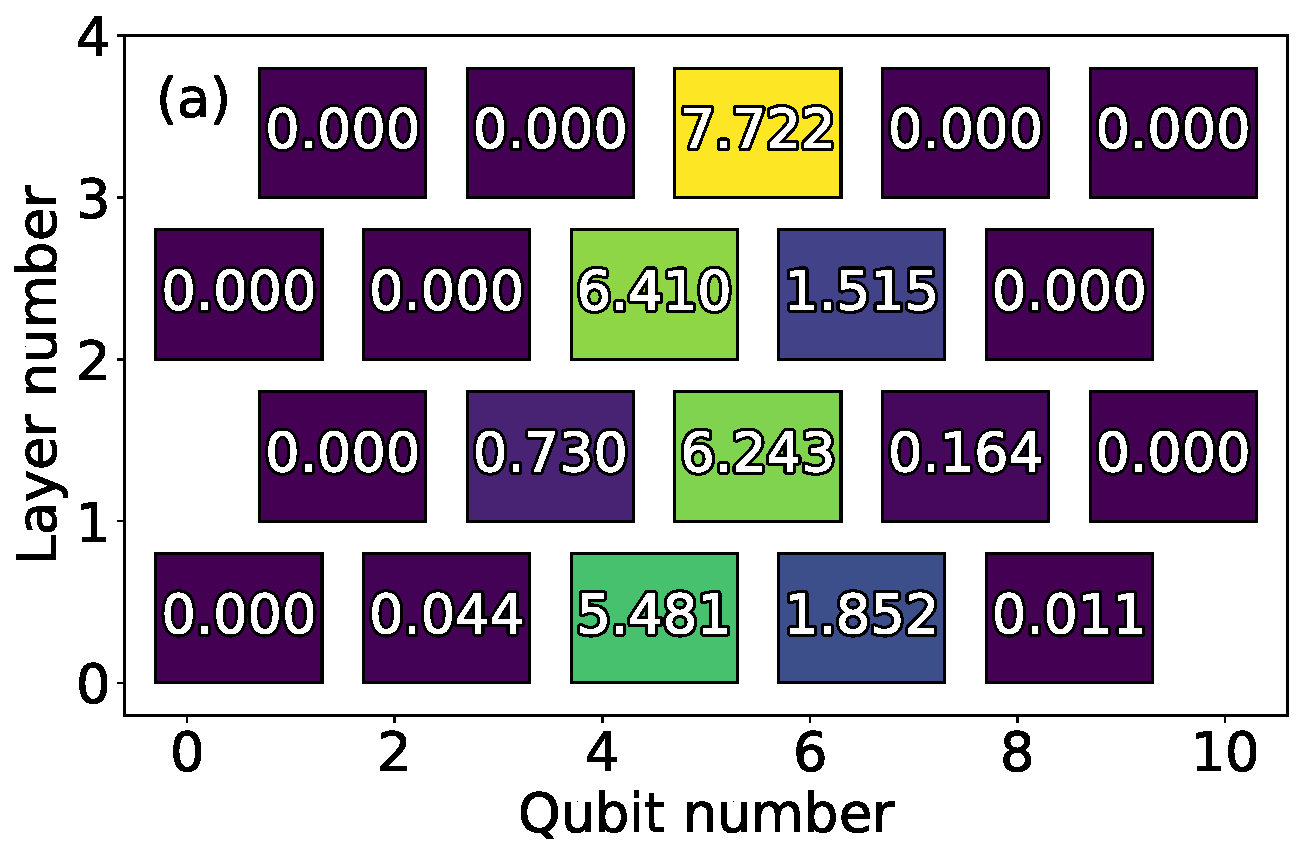
\includegraphics[width=\textwidth]{figures/X5_ising.pdf}
    \end{subfigure}\begin{subfigure}{.48\linewidth}
        \centering
        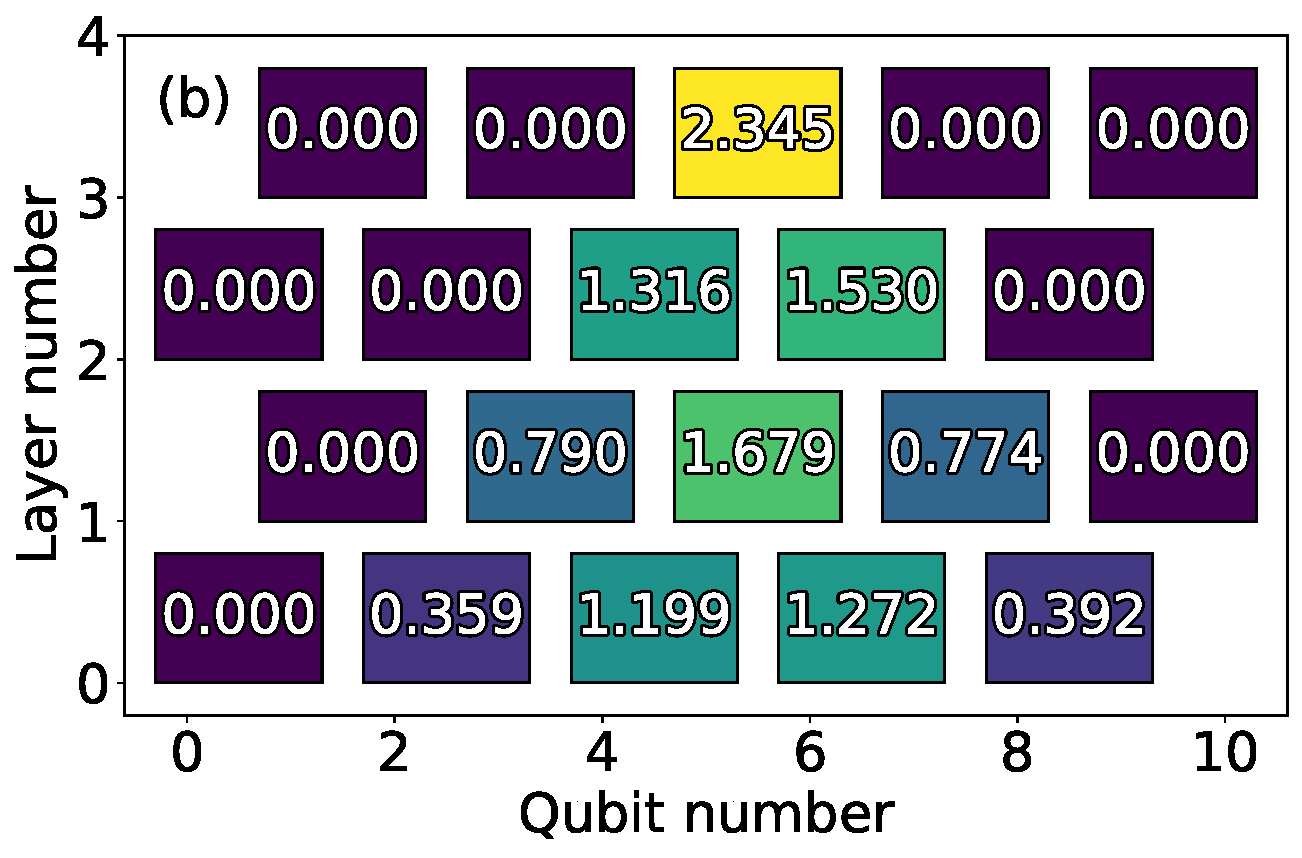
\includegraphics[width=\textwidth]{figures/X5_cartan.pdf}
    \end{subfigure}
    \begin{subfigure}{.48\linewidth}
        \centering
        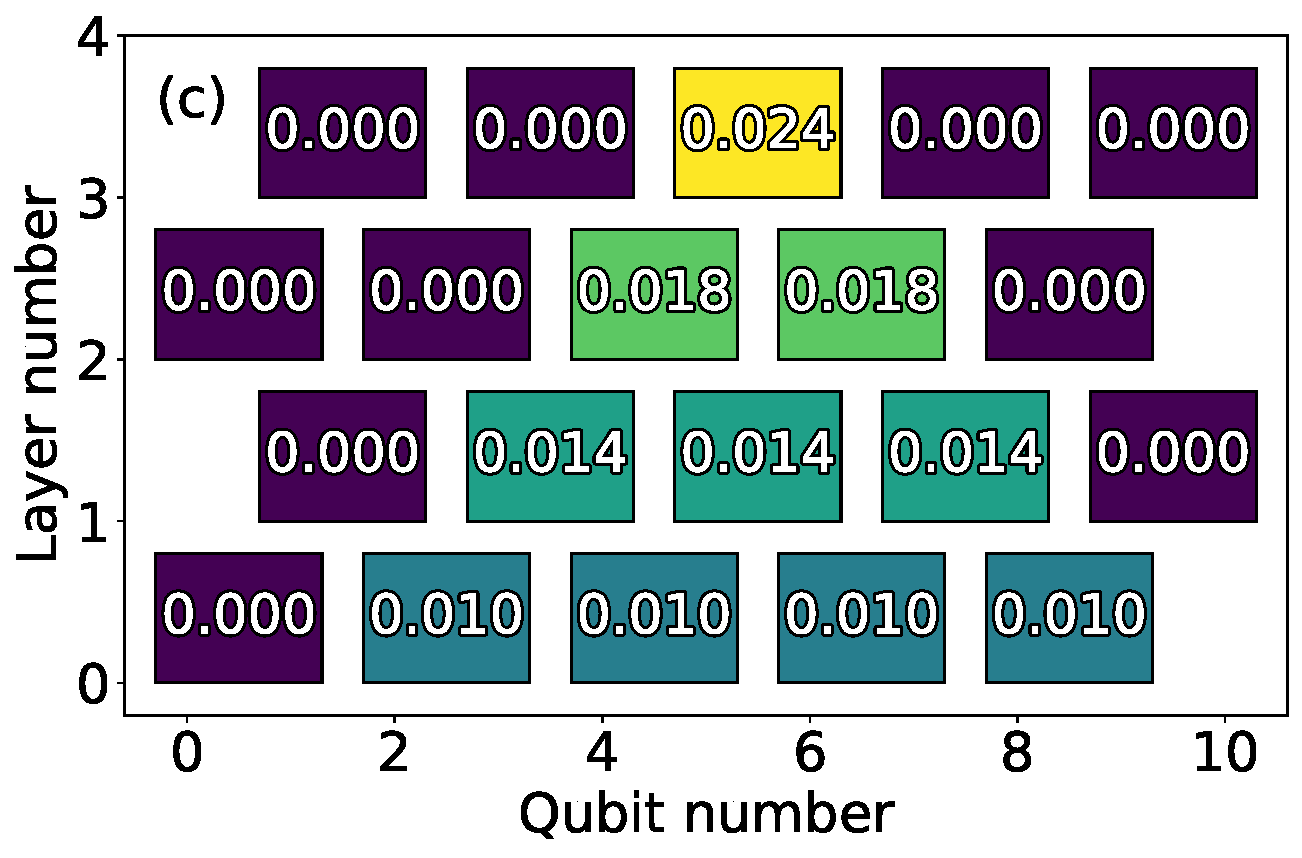
\includegraphics[width=\textwidth]{figures/X5_theory.pdf}
    \end{subfigure}
    \caption{Derivative variances for $H = X_5$, averaged over parameters in each ansatz block. The numbers in the boxes denote $\Var \partial_\theta E \cdot 100$. Qubit number 10 is identified with qubit number 0. (a) Numerical result for an ansatz with blocks of $X,Z,ZZ$ rotations. (b) Numerical result for blocks implemented according to the Cartan decomposition. (c) Lower bound given in Theorem \ref{thm:block_plateaus}. Reprinted from~\cite{uvarov_barren_2021}.}
    \label{fig:one-local}
\end{figure}

To estimate gradients, we used the following analytical procedure \cite{mitarai_quantum_2018,schuld_evaluating_2019}: let $f(\theta)$ be the cost function, and $\theta$ a parameter which is included in the quantum circuit in a gate like $\exp(\rmi F\theta / 2)$ for some Pauli operator $F$. Then the derivative w.r.t.\ this parameter is equal to $(f(\theta + \pi /2) - f(\theta - \pi / 2))/2$. The simulations assume noise-free conditions and use the statevector simulator provided by Qiskit~\cite{aleksandrowicz_qiskit:_2019}.

The first Hamiltonian we tested our predictions on is the single-qubit Hamiltonian $H = X_5$ acting on $n=10$ qubits. The qubits are enumerated starting from zero. 
For $N = 400$ samples, the derivative with respect to each parameter was evaluated, then the variances were averaged over each block. We performed two numerical experiments with different two-qubit blocks from Table \ref{tab:local_designs}: one with blocks of $X$, $Z$, and $ZZ$ rotations, and the other with blocks implemented according to the Cartan decomposition of $SU(4)$. The ansatz used was the checkerboard ansatz with ring connectivity. The result of the numerical test is shown in Fig.~\ref{fig:one-local}. 

\begin{figure}
    \centering
    \begin{subfigure}{.48\linewidth}
        \centering
        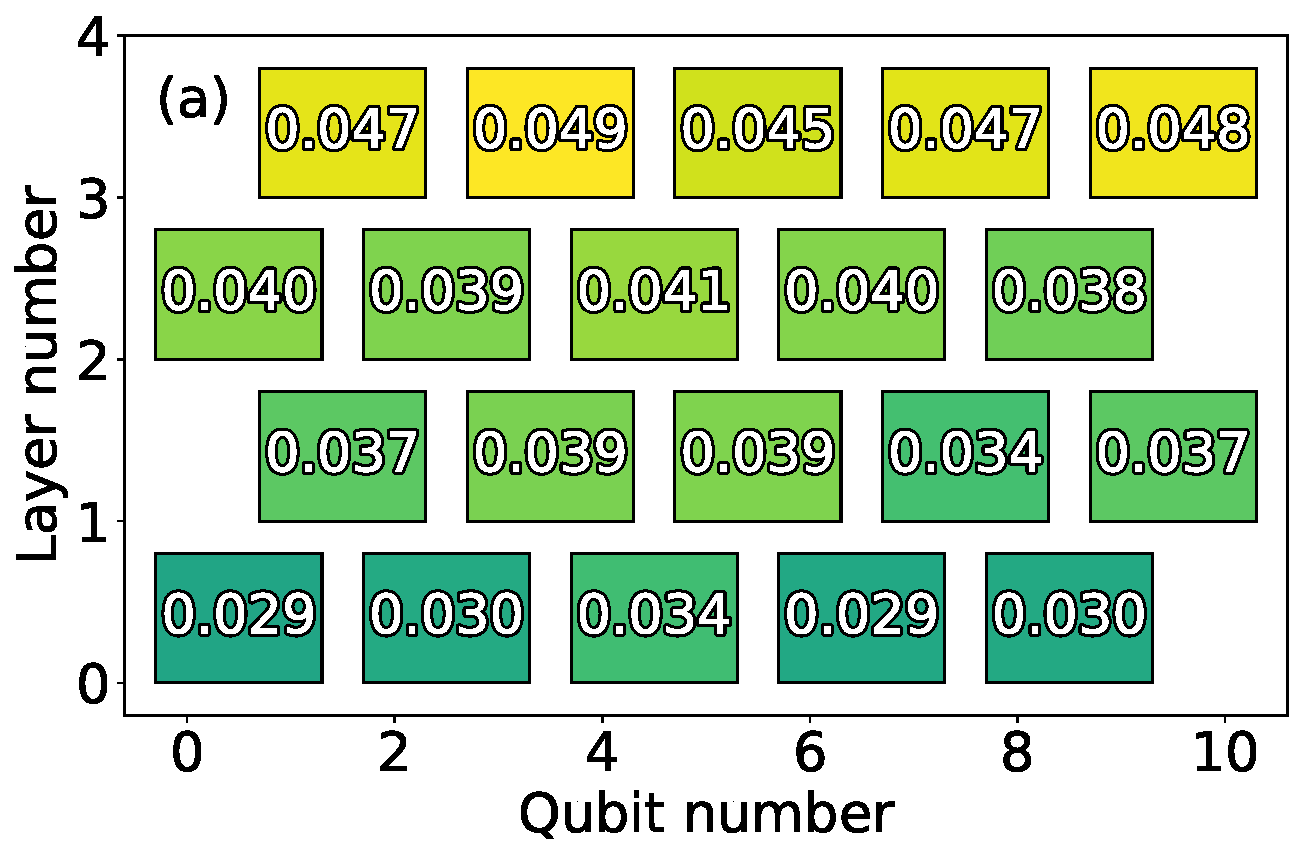
\includegraphics[width=\linewidth]{figures/dense_cartan.pdf}
    \end{subfigure}
    \begin{subfigure}{.48\linewidth}
        \centering
        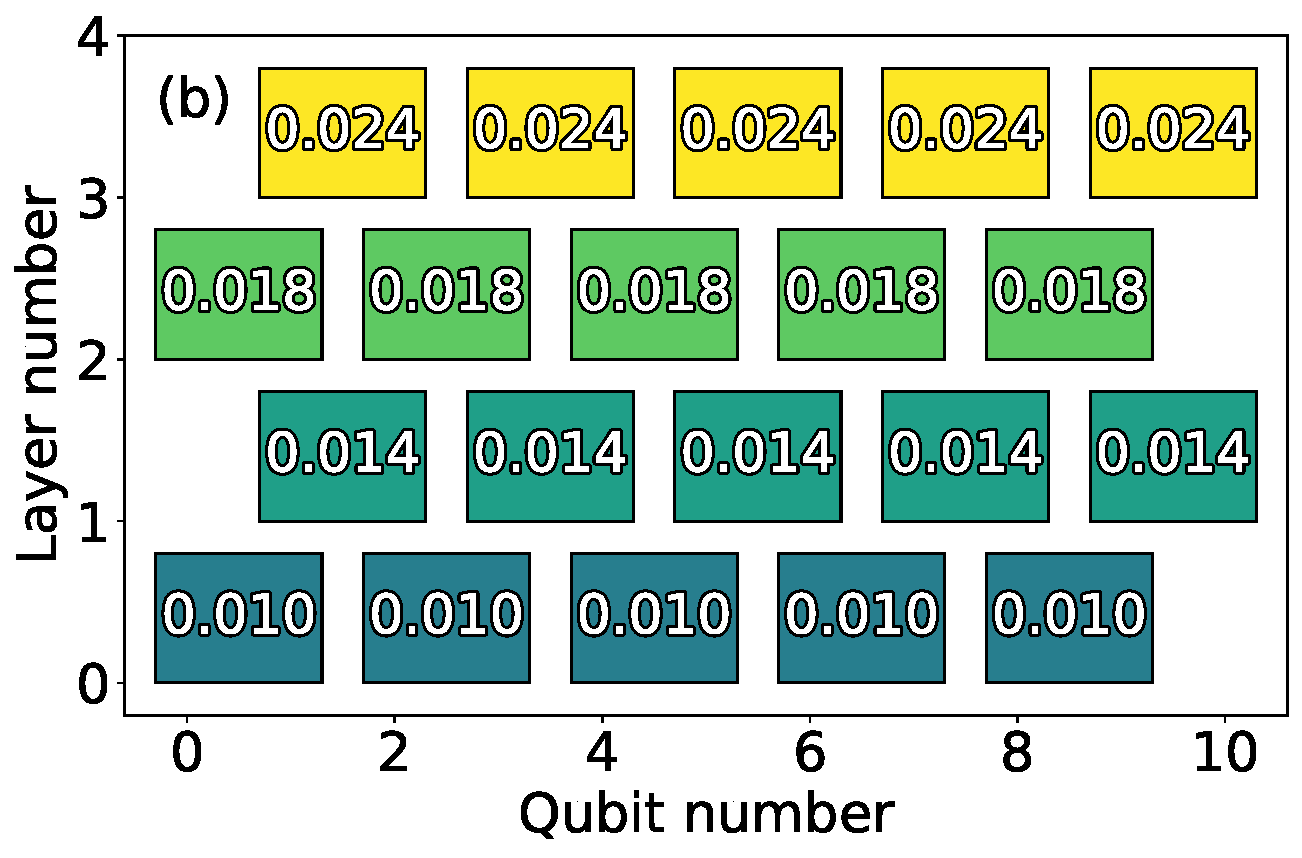
\includegraphics[width=\linewidth]{figures/dense_theory.pdf}
    \end{subfigure}
    \caption{Derivative variances for $H = X^{\otimes n}$, numerical estimate (a) and the lower bound (b). Reprinted from~\cite{uvarov_barren_2021}.}
    \label{fig:n-local}
\end{figure}

In both experiments, the causal cone structure is evident, as is evident the tendency of the gradients to decrease with the decreasing number of layer. However, the Cartan decomposed blocks show smoother results. This result is consistent with the fact that the first block type is further from a 2-design. The condition that the block can be further decomposed into two independent local 2-designs is also violated in the first case. Because of these factors, the gradients are uneven.

The theoretical lower bound is fulfilled by a large margin in both cases. The lower bound also does not catch the difference of gradients within one layer, which tend to be more significant in the middle of the causal cone as opposed to the edges of the cone, where the gradients are much smaller.

Figure \ref{fig:n-local} shows the results of a similar numerical test for $H = X^{\otimes n}$ for $n = 10$. Here, the ``Cartan decomposition'' blocks were used in the ansatz. As implied by the lower bound and in accordance with the results previously found in the literature \cite{cerezo_cost-function-dependent_2020}, this $n$-local Hamiltonian exhibits barren plateaus even for a very shallow ansatz.

According to \eqref{eq:paulis_decouple}, variances for a Hamiltonian consisting of several Pauli strings are equal to the sum of variances computed for each Pauli string independently. We tested that prediction on a pair of Hamiltonians $H_1 = X_4 X_5$, $H_2 = X_5 X_6$. In this test, the ansatz acts on 10 qubits and consists of 4 layers of ``Cartan decomposition'' blocks. The variances for $H_1$ and $H_2$ separately are shown as a stacked bar chart in Fig.~\ref{fig:additive}a. Each bar corresponds to a parameter $\theta_i$ in the ansatz. Fig.~\ref{fig:additive}b shows the variances for $H_1 + H_2$. The qualitative agreement between the graphs is evident, and the differences for each parameter of the ansatz (shown in Fig.~\ref{fig:additive_delta}) are close to zero, up to the standard errors of the samples.


\subsection{Alternative ansatz architectures}
\label{subsec:alt_ansatz}

The width of the causal cone depends on the ansatz structure. Conversely, some ansatz structures may be less prone to barren plateaus. We performed the same numerical tests for two more circuit architectures that are better suited for NISQ devices.

\begin{figure}
    \centering
    \begin{subfigure}{.48\linewidth}
        \centering
        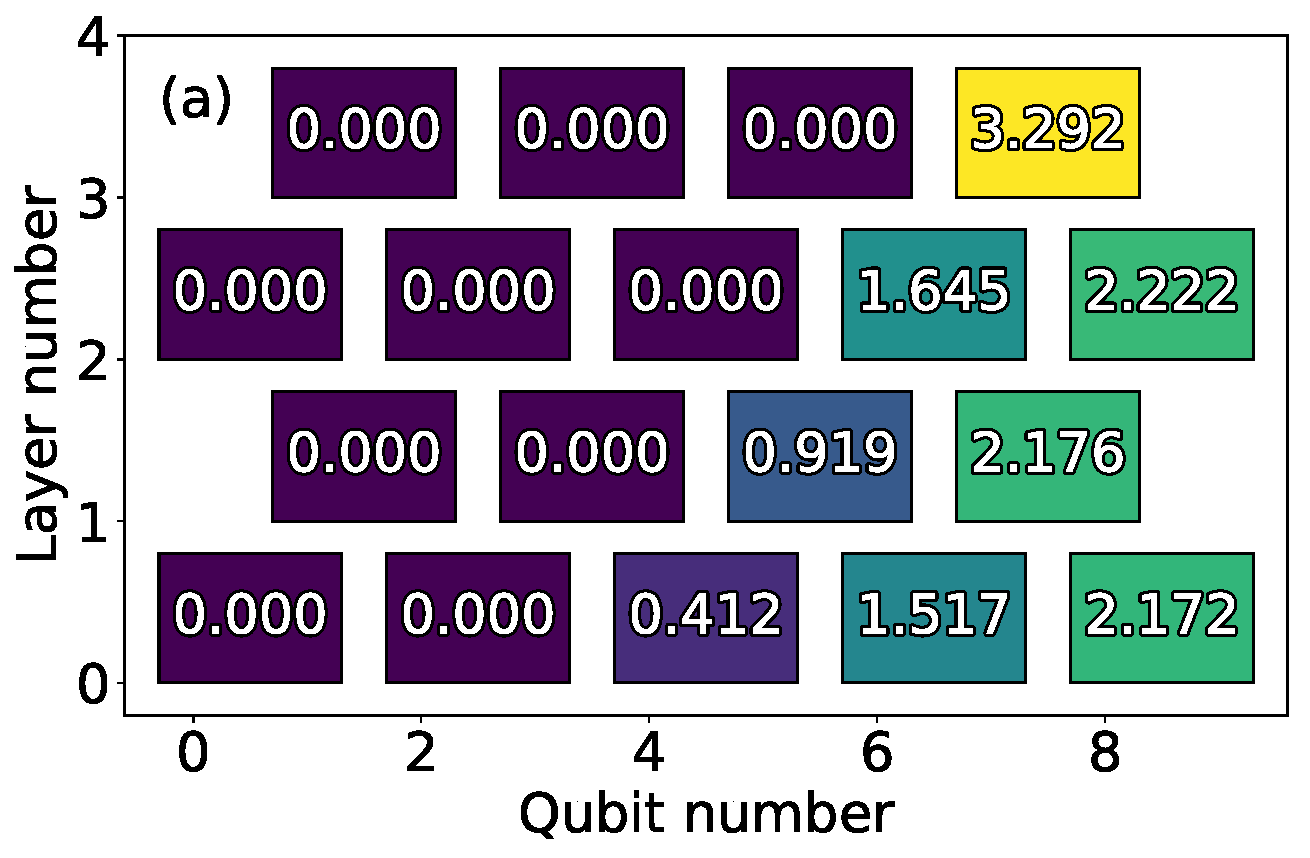
\includegraphics[width=\linewidth]{figures/line_endpoint.pdf}
    \end{subfigure}
    \begin{subfigure}{.48\linewidth}
        \centering
        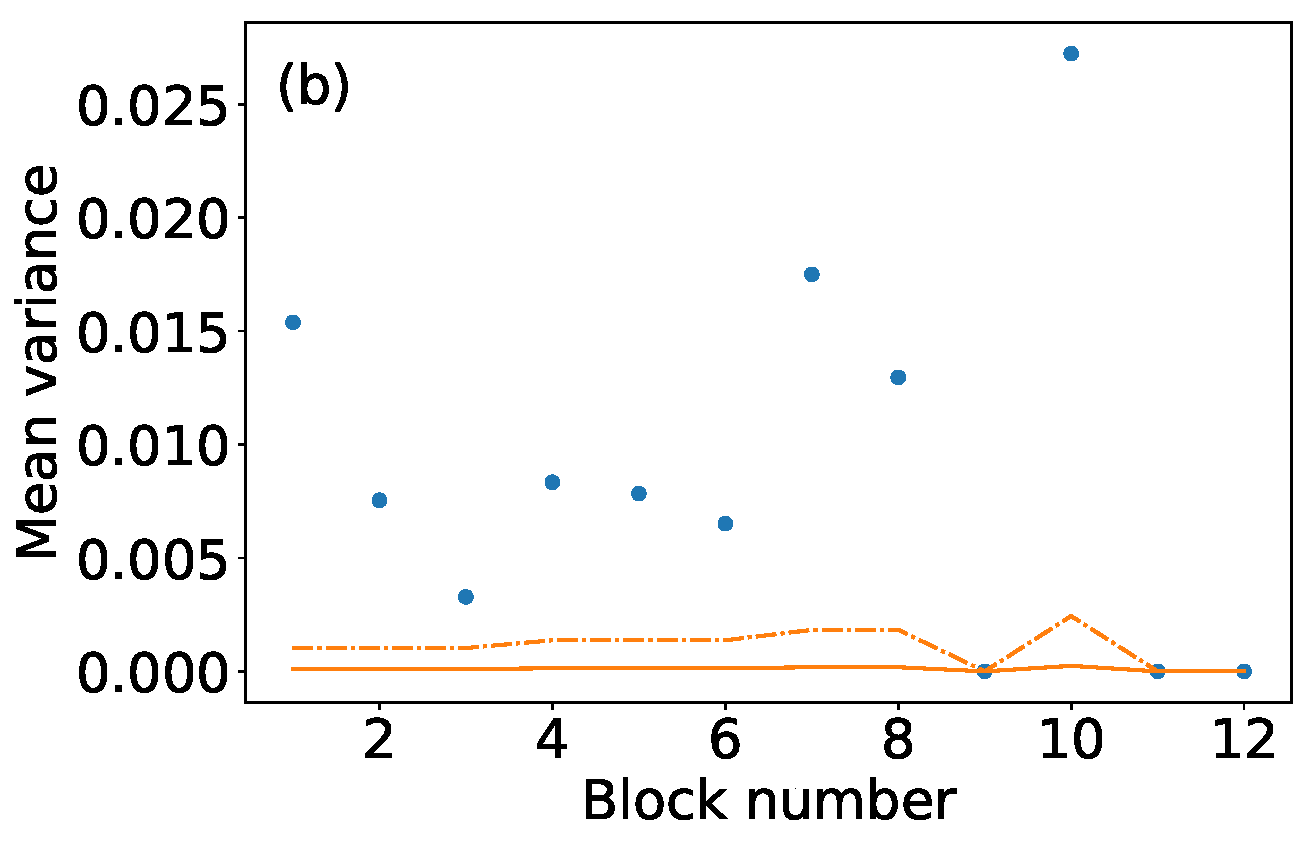
\includegraphics[width=\linewidth]{figures/lattice_scatter.pdf}
    \end{subfigure}
    \caption{Blockwise averaged values of derivative variances with respect to one-local Pauli strings. (a) Numerical result for a line-connected checkerboard ansatz. (b) Numerical result for a two-dimensional lattice ansatz. Dots: numerical values, line: lower bound,  dot-dashed line: lower bound multiplied by 10. Reprinted from~\cite{uvarov_barren_2021}.}
    \label{fig:alt_connect}
\end{figure}


\subsubsection{Checkerboard with open boundary conditions}

For certain quantum computing platforms, e.g.~Calcium ions and Rydberg atoms, it is easiest to arrange qubits in a line and perform entangling gates acting on adjacent qubits. Unlike ring connectivity, this structure does not use direct coupling of the first qubit with the last qubit. Thus, the qubits closer to the edge will have narrower causal cones, and possibly higher values of the gradients. Fig.~\ref{fig:alt_connect}a shows the behavior of derivatives for such an architecture, for $H = X_8$. In comparison with the ring connectivity (Fig. \ref{fig:one-local}b), the gradient variances are significantly larger.

\begin{figure}
    \centering
    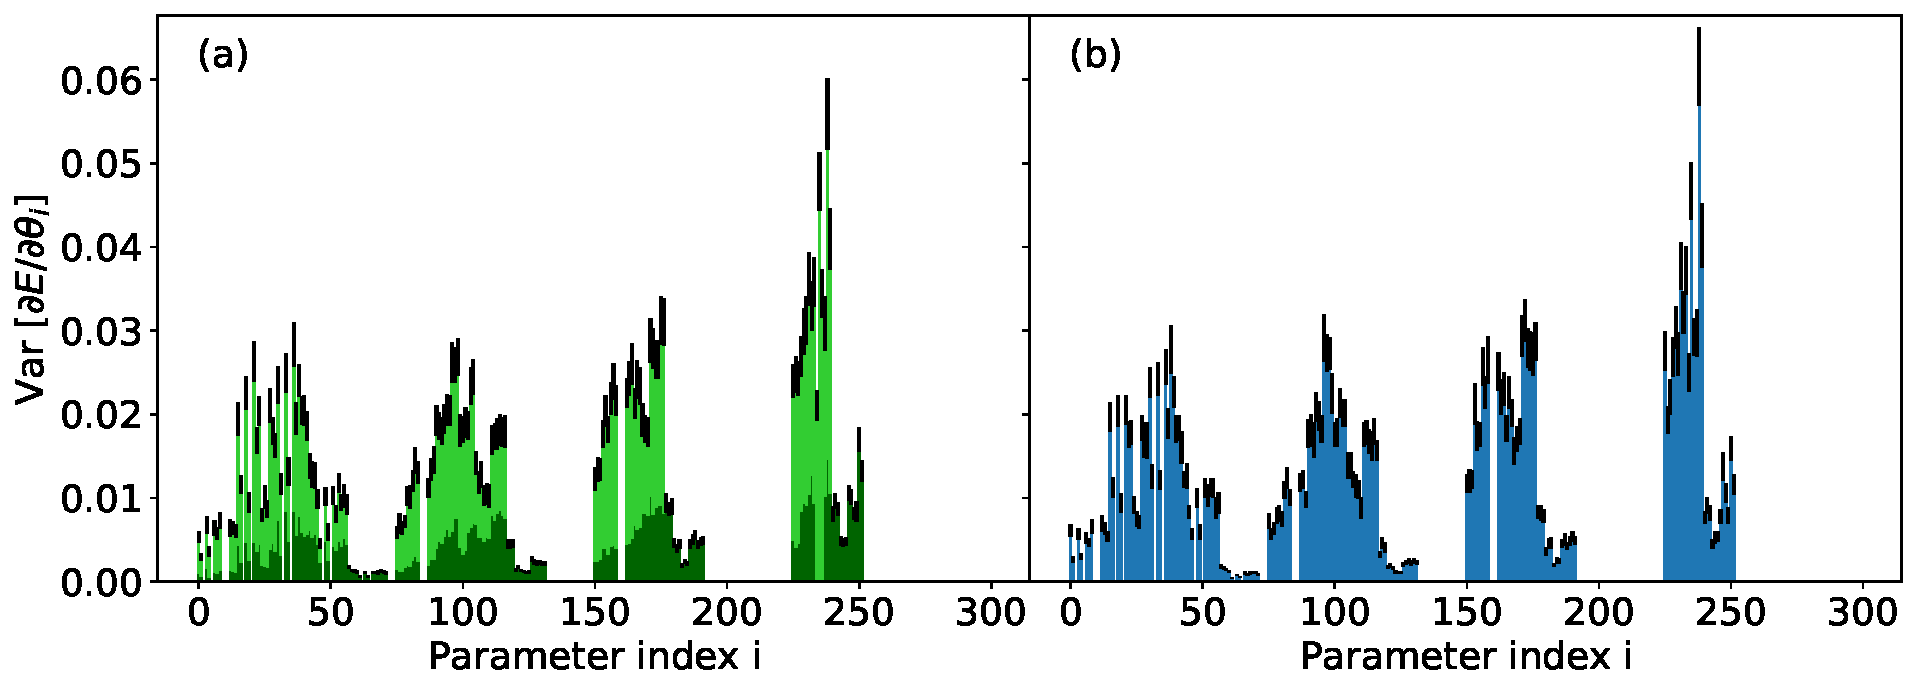
\includegraphics[width=\linewidth]{figures/sums_comparison_separate.pdf}
    \caption{Variances of the cost function derivatives with respect to different ansatz parameters for $H_1 = X_5 X_6$, $H_2 = X_4 X_5$ (a), and their sum $H_1 + H_2$ (b). Reprinted from~\cite{uvarov_barren_2021}.}
    \label{fig:additive}
\end{figure}

\begin{figure}
    \centering
    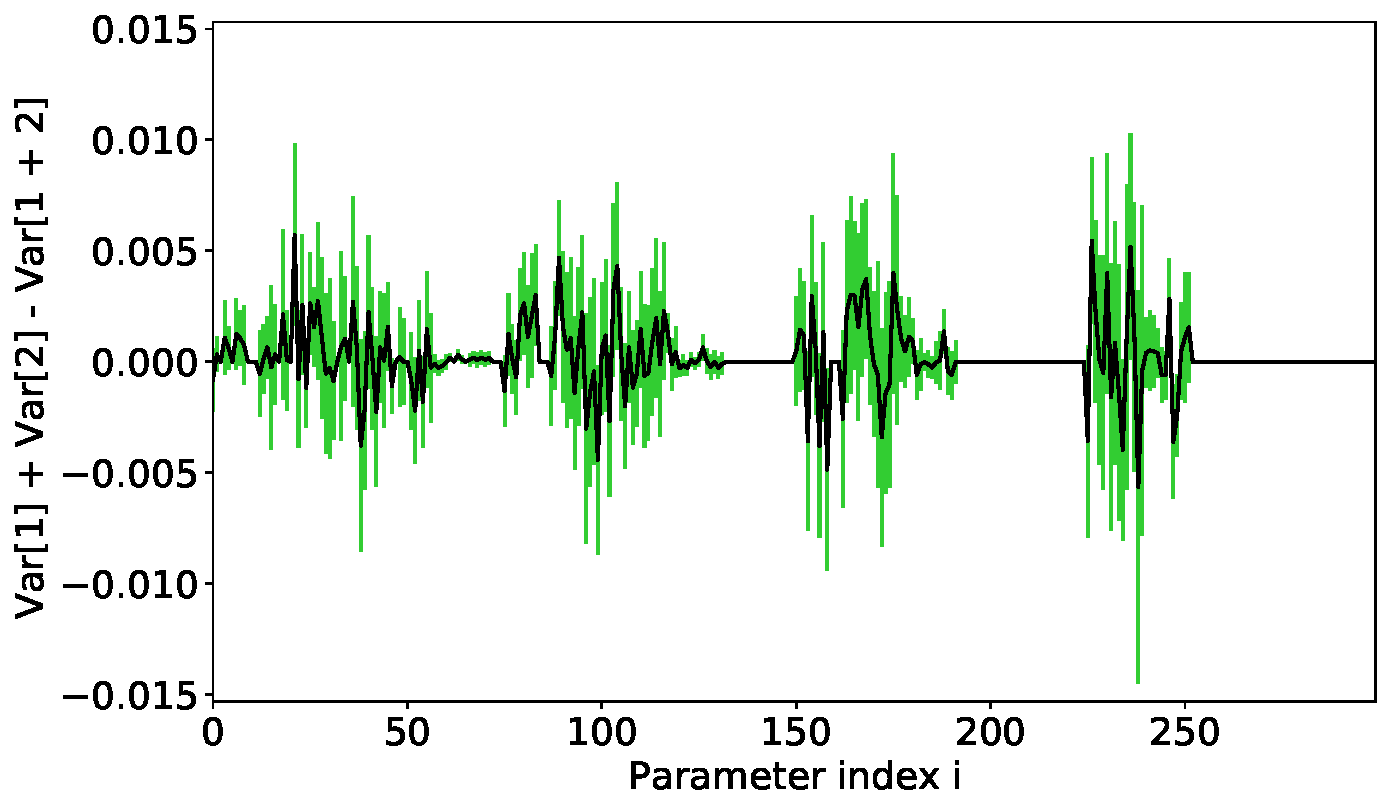
\includegraphics[width=0.7\linewidth]{figures/sums_comparison_difference.pdf}
    \caption{Difference between the variances plotted in Fig.~\ref{fig:additive}. Error bars denote one standard error. Reprinted from~\cite{uvarov_barren_2021}.}
    \label{fig:additive_delta}
\end{figure}


\subsubsection{Two-dimensional lattice}

We also tested the predictions of Theorem \ref{thm:block_plateaus} on a two-dimensional $3 \times 3$ lattice. The two-dimensional lattice ansatz is constructed as follows. The first layer of the ansatz is schematically depicted in Fig.~\ref{fig:2d_ansatz_scheme}. Every next layer is obtained from the last by rotating the layout 90 degrees clockwise. The two-dimensional ansatz consisted of four layers of two-qubit blocks. 

The numerical values of the derivative variances, as well as their lower bounds, are depicted in Fig.~\ref{fig:alt_connect}b. The causal cone structure for this ansatz is more convoluted, but it is possible to tell that some ansatz blocks are not included in the causal cone, and hence, the derivative over their parameters is equal to zero. 

\begin{figure}
    \centering
    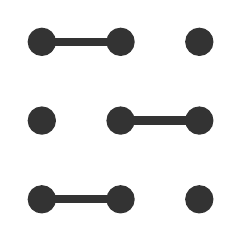
\begin{tikzpicture}[thick]
    \node at ( 0,0) [circle,draw=black!80,fill=black!80] {};
    \node at ( 0,1) [circle,draw=black!80,fill=black!80] {};
    \node at ( 0,2) [circle,draw=black!80,fill=black!80] {};
    \node at ( 1,0) [circle,draw=black!80,fill=black!80] {};
    \node at ( 1,1) [circle,draw=black!80,fill=black!80] {};
    \node at ( 1,2) [circle,draw=black!80,fill=black!80] {};
    \node at ( 2,0) [circle,draw=black!80,fill=black!80] {};
    \node at ( 2,1) [circle,draw=black!80,fill=black!80] {};
    \node at ( 2,2) [circle,draw=black!80,fill=black!80] {};
    
    \draw [draw=black!80,line width=3] (0,0) -- (1,0);
    \draw [draw=black!80,line width=3] (1,1) -- (2,1);
    \draw [draw=black!80,line width=3] (0,2) -- (1,2);
    \end{tikzpicture}    
    \caption{Connectivity of one layer in the 2D lattice ansatz. Other layers are formed by rotating this pattern by 90 degrees. Reprinted from~\cite{uvarov_barren_2021}.}
    \label{fig:2d_ansatz_scheme}
\end{figure}


% \section{Meaning of the operator 2-norm of the TPE}
% \label{sec:2-norm_TPE}




% \section{Structure of the two-dimensional lattice ansatz}
% \label{sec:2d_ansatz}

\section{Discussion}
Given a Hamiltonian, we can now estimate its susceptibility to the barren plateaus. One can hence preprocess Hamiltonians in order to make the optimization more viable. For example, a method similar to that of Ref.~\cite{ryabinkin_iterative_2020} could be employed.

Our results indicate that the severity of plateaus also depends on the structure of the ansatz. This may mean that some hardware topologies are more suited for VQE than others. For example, our numerical tests demonstrate that in line connectivity of the qubits, the gates on the edges are potentially less prone to vanishing derivatives than those in the middle.

The numerical tests provided in this chapter can be implemented in hardware as well. The computational cost of simulating a quantum computer using the best known methods is exponential either in time or in memory, while estimation of the gradients in quantum hardware (up to fixed absolute tolerance) is linear in the number of ansatz parameters, and possibly even sub-linear in the cardinality of the problem Hamiltonian, if clever simultaneous measurement strategies are used \cite{verteletskyi_measurement_2020}. 

At the first glance, the barren plateaus phenomenon looks like a ``no-go'' result that prevents training any quantum circuits of sufficiently high depth. However, since the condition is that the parameters are random, it is more of a caution to not initialize circuits at random. This was first noted in \cite{grant_initialization_2019}, where the authors proposed initializing most gates with zero rotation angles. In this situation, the starting point is not chosen uniformly randomly across the entire search space, but instead it is sampled from a small neighborhood of zero. 

Other plentiful variants of VQE (see Section \ref{sec:vqe_variants}) rely on dynamically adjusting the ansatz. This can also be seen as a convoluted ``initialization strategy'': when the process produces a long ansatz, it already suggests a good starting point. 

% In Chapter \ref{chap:vqe_numerics}, we observed that the onset of barren plateaus for an ansatz consisting of particle-conserving gates, despite clear evidence that such an ansatz is not a 2-design. As we discussed earlier, this may imply that such an ansatz is an approximate 2-design when restricted to the particle number subspace.